%definira klasu dokumenta 
\documentclass[12pt]{report} 

%prostor izmedu naredbi \documentclass i \begin{document} se zove uvod. U njemu se nalaze naredbe koje se odnose na cijeli dokument
	
%osnovni LaTex ne može riješiti sve probleme, pa se koriste različiti paketi koji olakšavaju izradu željenog dokumenta
\usepackage[croatian]{babel} 
\usepackage{amssymb}
\usepackage{amsmath}
\usepackage{txfonts}
\usepackage{mathdots}
\usepackage{titlesec}
\usepackage{array}
\usepackage{lastpage}
\usepackage{etoolbox}
\usepackage{tabularray}
\usepackage{color, colortbl}
\usepackage{adjustbox}
\usepackage{geometry}
\usepackage[classicReIm]{kpfonts}
\usepackage{hyperref}
\usepackage{fancyhdr}

\usepackage{float}
\usepackage{setspace}
\restylefloat{table}


\patchcmd{\chapter}{\thispagestyle{plain}}{\thispagestyle{fancy}}{}{} %redefiniranje stila stranice u paketu fancyhdr

%oblik naslova poglavlja
\titleformat{\chapter}{\normalfont\huge\bfseries}{\thechapter.}{20pt}{\Huge}
\titlespacing{\chapter}{0pt}{0pt}{40pt}


\linespread{1.3} %razmak između redaka

\geometry{a4paper, left=1in, top=1in,}  %oblik stranice

\hypersetup{ colorlinks, citecolor=black, filecolor=black, linkcolor=black,	urlcolor=black }   %izgled poveznice


%prored smanjen između redaka u nabrajanjima i popisima
\newenvironment{packed_enum}{
\begin{enumerate}
	\setlength{\itemsep}{0pt}
	\setlength{\parskip}{0pt}
	\setlength{\parsep}{0pt}
}{\end{enumerate}}

\newenvironment{packed_item}{
\begin{itemize}
	\setlength{\itemsep}{0pt}
	\setlength{\parskip}{0pt}
	\setlength{\parsep}{0pt}
}{\end{itemize}}




%boja za privatni i udaljeni kljuc u tablicama
\definecolor{LightBlue}{rgb}{0.9,0.9,1}
\definecolor{LightGreen}{rgb}{0.9,1,0.9}

%Promjena teksta za dugačke tablice
\DefTblrTemplate{contfoot-text}{normal}{Nastavljeno na idućoj stranici}
\SetTblrTemplate{contfoot-text}{normal}
\DefTblrTemplate{conthead-text}{normal}{(Nastavljeno)}
\SetTblrTemplate{conthead-text}{normal}
\DefTblrTemplate{middlehead,lasthead}{normal}{Nastavljeno od prethodne stranice}
\SetTblrTemplate{middlehead,lasthead}{normal}

%podesavanje zaglavlja i podnožja

\pagestyle{fancy}
\lhead{Programsko inženjerstvo}
\rhead{GlobeRunner}
\lfoot{CrnePatike}
\cfoot{stranica \thepage/\pageref{LastPage}}
\rfoot{\today}
\renewcommand{\headrulewidth}{0.2pt}
\renewcommand{\footrulewidth}{0.2pt}


\begin{document} 



\begin{titlepage}
	\begin{center}
		\vspace*{\stretch{1.0}} %u kombinaciji s ostalim \vspace naredbama definira razmak između redaka teksta
		\LARGE Programsko inženjerstvo\\
		\large Ak. god. 2022./2023.\\
		
		\vspace*{\stretch{3.0}}
		
		\huge GlobeRunner\\
		\Large Dokumentacija, Rev. \textit{1}\\
		
		\vspace*{\stretch{12.0}}
		\normalsize
		Grupa: \textit{Crne patike}\\
		Voditelj: \textit{Robert Kunštek}\\
		
		
		\vspace*{\stretch{1.0}}
		Datum predaje: \textit{18. 11. 2022}\\
		
		\vspace*{\stretch{4.0}}
		
		Nastavnik: \textit{Hrvoje Nuić}\\
		
	\end{center}
	
	
\end{titlepage}


\tableofcontents


\chapter{Dnevnik promjena dokumentacije}

%\textbf{\textit{Kontinuirano osvježavanje}}\\


\begin{longtblr}[
	label=none
	]{
		width = \textwidth, 
		colspec={|X[2]|X[13]|X[3]|X[3]|}, 
		rowhead = 1
	}
	\hline
	\textbf{Rev.}	& \textbf{Opis promjene/dodatka} & \textbf{Autori} & \textbf{Datum}\\[3pt] \hline
	0.1 & Napravljen predložak, dodani funkcionalni zahtjevi.	& Svi & 02.11.2022. 		\\[3pt] \hline
	0.2	& Dodani obrasci uporabe & Svi & 11.11.2022. 	\\[3pt] \hline 
	0.3	& Dodan početak 4. poglavlja & Robert Kunštek & 14.11.2022. 	\\[3pt] \hline 
	0.4 & Dodano poglavlje 4.1 & Marela Arambašić & 15.11.2022. \\[3pt] \hline 
	0.5 & Dodano poglavlje 2 & Mateo Kopačević & 15.11.2022. \\[3pt] \hline 
	0.6 & Dodano poglavlje 3.2, ispravljeno poglavlje 2 & Mateo Kopačević  & 15.11.2022. \\[3pt] \hline 
	0.7 & Dodan opis za 3.1.2 i ispravljen UC-14 & Luka Arambašić & 15.11.2022. \\[3pt] \hline 
	0.8 & Dodani sekvencijski dijagrami & Luka Arambašić & 16.11.2022. \\[3pt] \hline 
	0.9 & Ispravljeno poglavlje 4.1 & Marela Arambašić & 16.11.2022. \\[3pt] \hline
	1.0 & Dovršavanje prve verzije 4.1 & Robert Kunštek & 18.11.2022. \\[3pt] \hline
\end{longtblr}


%\textit{Moraju postojati glavne revizije dokumenata 1.0 i 2.0 na kraju prvog i drugog ciklusa. Između tih revizija mogu postojati manje revizije već prema tome kako se dokument bude nadopunjavao. Očekuje se da nakon svake značajnije promjene (dodatka, izmjene, uklanjanja dijelova teksta i popratnih grafičkih sadržaja) dokumenta se to zabilježi kao revizija. Npr., revizije unutar prvog ciklusa će imati oznake 0.1, 0.2, …, 0.9, 0.10, 0.11.. sve do konačne revizije prvog ciklusa 1.0. U drugom ciklusu se nastavlja s revizijama 1.1, 1.2, itd.}

\chapter{Opis projektnog zadatka}
		
		
Cilj ovog projekta je razvoj programske podrške za stvaranje interaktivne web aplikacije „GlobeRunner“  koja omogućuje igračima međusobnu borbu kartama koje su sakupili na različitim stvarnim lokacijama svijeta. Moguće lokacije koje igrači mogu posjetiti su gradovi, naselja, vrhovi planina, umjetničke instalacije, izvori vode, planinarski domovi i sl.
Svaki se neregistrirani korisnik za pristup aplikaciji može prijaviti u već postojeći račun pri čemu je potrebno upisati korisničko ime i lozinku ili stvoriti novi račun. Za stvaranje novog računa potrebni su sljedeći podaci:
		\begin{packed_item}
			\item {Korisničko ime}
			\item {Fotografija}
			\item {E - mail adresa}
			\item {Lozinka}
		\end{packed_item}
		
Pri registraciji korisnik može odabrati jednu od uloga: igrač ili kartograf. Naknadno se može dodijeliti uloga administratora. Registracija nije prihvatljiva ako je zadano korisničko ime ili e – mail adresa već postojećeg računa ili nepostojeća e – mail adresa. Nakon popunjavanja podataka za registraciju korisniku se na e – mail šalje link kojim potvrđuje svoj račun. Ako se korisnik odluči za ulogu kartografa dodatno je potrebna potvrda administratora te dodatni podaci za primanje naknade:
		\begin{packed_item}
			\item {IBAN računa za uplatu}
			\item {Fotografija osobne iskaznice}
		\end{packed_item}
	

Administrator će odbiti registraciju kartografa ako je predan nepostojeći IBAN ili je utvrdio neispravnost podataka.\\

\textit {\underbar{Karta (Lokacija)}} je glavni element igre kojom se igrači međusobno bore. Svaka karta ima naziv, opis, fotografiju i jačinu. Što je lokacija šira i lakše dostupna, to je karta slabija (npr. gradovi su slabiji od muzeja u tim gradovima). Karta nakon svake upotrebe slabi do nule nakon čega više nije upotrebljiva. Cilj ovoga je potaknuti igrače da putuju svijetom i skupljaju što više karata.\\
 
\textit {\underbar{Igrač}} je svaki korisnik koji aktivno skuplja karte i sudjeluje u borbama. Za ispravno i uspješno korištenje aplikacije mora imati uključen GPS.
Za vrijeme igre igraču su vidljivi svi aktivni igrači unutar 50 km s kojima može ući u borbu. Omogućeno mu je pregledavanje profila igrača što uključuje sakupljene karte, poredak u odnosu na ostale igrače te statistiku temeljenu na zadnjih 10 borbi.
Također može pregledati globalnu statistiku svih odigranih borbi, globalnu statistiku svih lokacija te poredak ostalih igrača. Igrač može sakupljati nove karte tako što posjeti određenu lokaciju, također ako je dovoljno iskusan i visoko na poretku može prijaviti novu lokaciju u blizini dodavajući sve potrebne podatke lokacije. Prije ulaska u borbu s drugim igračem, igrač može birati skup karata s kojim će se boriti.\\

\textit {\underbar{Borba}} se odvija tako što 2 igrača naizmjenice vuku po jednu kartu iz svog skupa. Karta s većom jačinom pobjeđuje te igrač čija je karta pobijedila dobiva bod. Nakon što su sve karte iskorištene igrač s više bodova pobjeđuje borbu.\\

\textit {\underbar {Kartograf}} održava i uređuje bazu sustava u koju zapisuje nove prijavljene lokacije.
Kartograf mora osigurati ispravnost zahtjeva za prijavu novih lokacija koje su igrači podnijeli. Može pristupiti popisu svih trenutno aktivnih zahtjeva. Lokacije za koje su podneseni zahtjevi vidljivi su mu na karti a on ih može prihvatiti, urediti, odbiti ili označiti da je potrebna potvrda s terena. Ako označi da je potrebna potvrda s terena može dodatno odlučiti da će ih on sam potvrditi i odlazi na lokaciju najkraćim putem.\\

\textit {\underbar {Administrator}} je korisnik s najviše ovlasti u igri koji ima pristup gotovo svim dijelovima sustava. Sadrži sve mogućnosti koje posjeduju igrači te kartografi, a uz to dodatno mora potvrditi svaku novu registraciju kartografa, može vidjeti i uređivati popis svih korisnika te njihovih osobnih podataka, privremeno isključiti igrača iz igre te može uređivati i postojeće lokacije u igri.\\

Svi podaci korisnika i lokacija pohranjuju se u bazu podataka kojom upravljaju kartografi i administratori. Baza podataka se početno puni određenim osnovnim lokacijama te se naknadno dopunjuje registracijama igrača i prijavama lokacija.\\

Aplikacija potiče zdrav život, zabavu i istraživanje svijeta te ju može koristiti bilo tko. Osim što je aplikacija zamišljena kao interaktivna igra, zanemarujući aspekt borbe može se koristiti kao bilježnik lokacija koje se standardno ne prikazuju na popularnijim kartama kao što su Google Karte i sl. Korisnici mogu istraživati neistražene, manje poznate ili čak opasne lokacije te bilježiti informacije i dodavati lokacije u kartu kako bi ostali korisnici znali što se gdje nalazi. Najčešći korisnici bi bili planinari, istraživači teško dostupnih mjesta (prašume, špilje, pustinje, snježna područja i sl.). Jednostavno mogu planirati i dokumentirati svoja putovanja i obzirom da tehnika računanja najkraćeg puta postoji (u vidu kartografa), ostali korisnici bi uvijek mogli najkraćim putem doći do lokacije.\\

Jedan primjer aplikacije koja je izrađena na sličan način kao ovaj projekt jest nedavno popularna mobilna aplikacija „Pokémon GO“. Aplikacija se zasniva na prikupljanju čarobnih bića poznatih kao Pokémoni prolazeći kroz stvarne lokacije u stvarnom vremenu (Slika 2.1). Nakon što se susretne jedan Pokémon koji se može nasumično stvoriti u blizini ili na popularnim lokacijama u lokanoj sredini, igrač hvata biće bacajući kuglu (Poké Ball). Uhvaćena bića mogu se trenirati i evoluirati te se može ulaziti u borbu s drugim igračima (Slika 2.2). Konceptualno razlika je samo u broju uloga; postoji samo jedna uloga, uloga igrača.

			
		
		%unos slike
		\begin{figure}[H]
			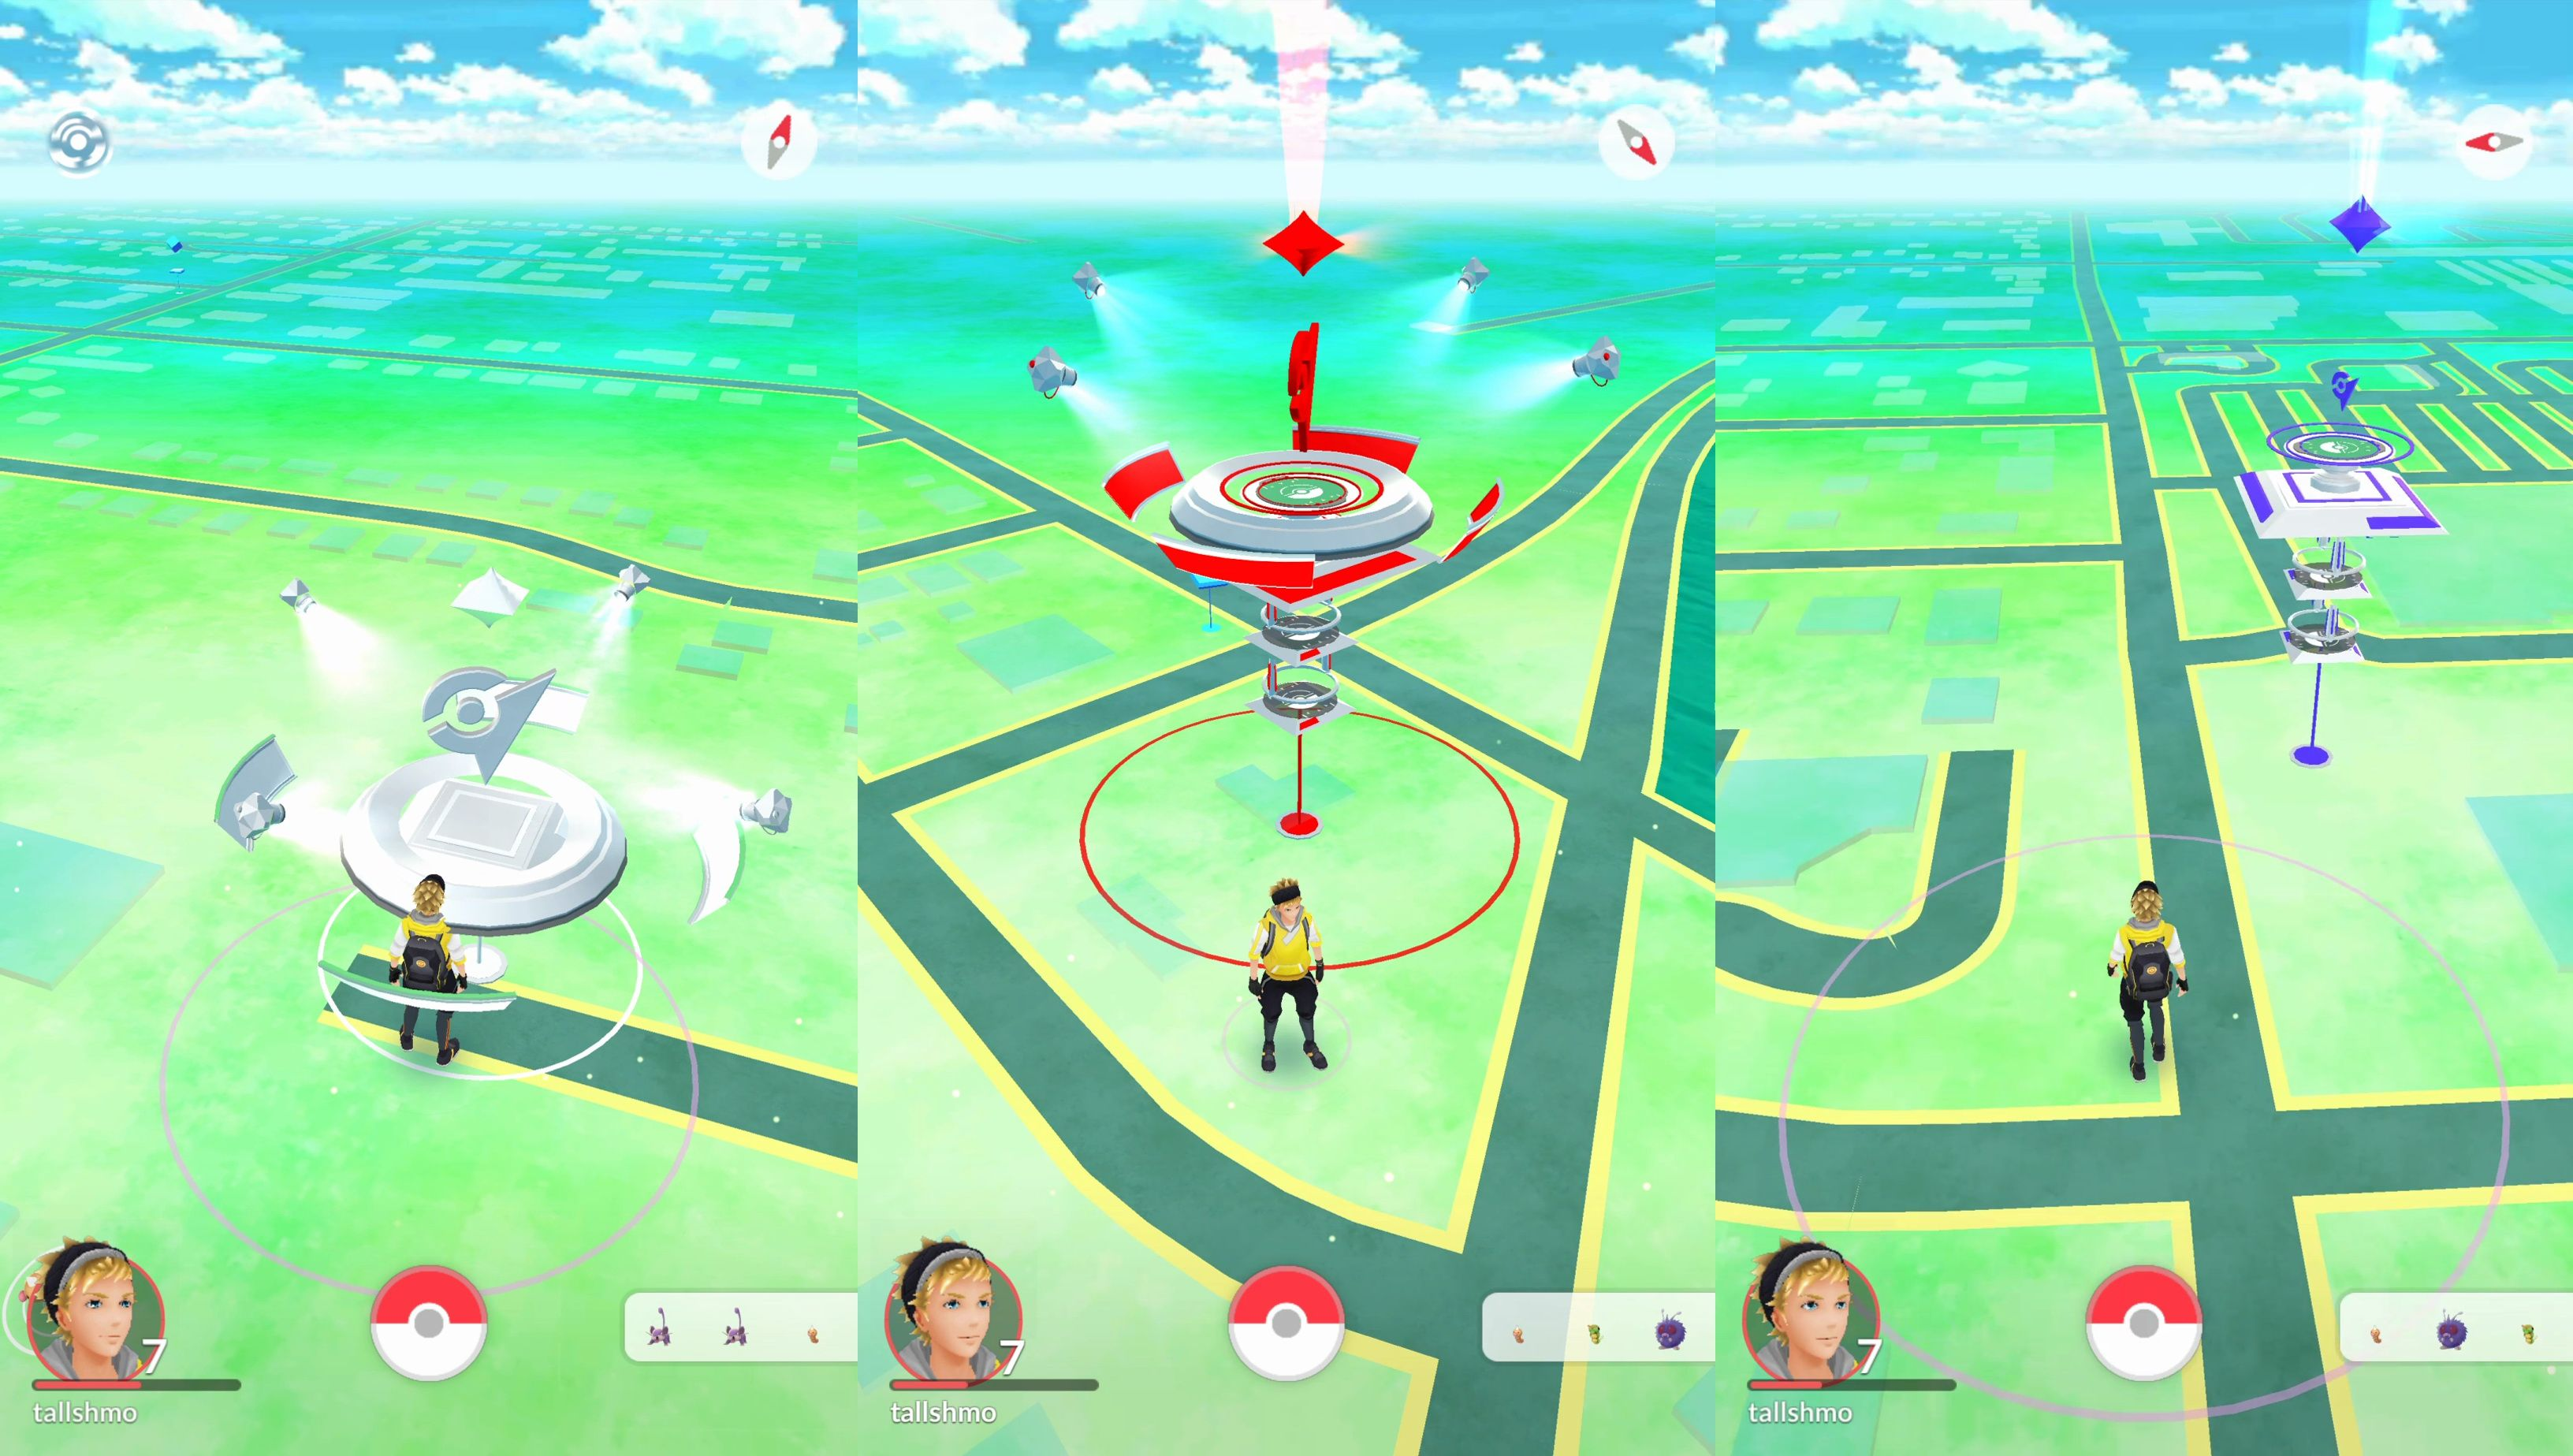
\includegraphics[width=\textwidth]{slike/Slika2.1.JPG} %veličina u odnosu na širinu linije
			\caption{Primjer karte u Pokemon GO}
			\label{fig:promjene1} %label mora biti drugaciji za svaku sliku
		\end{figure}
		
		\begin{figure}[H]
			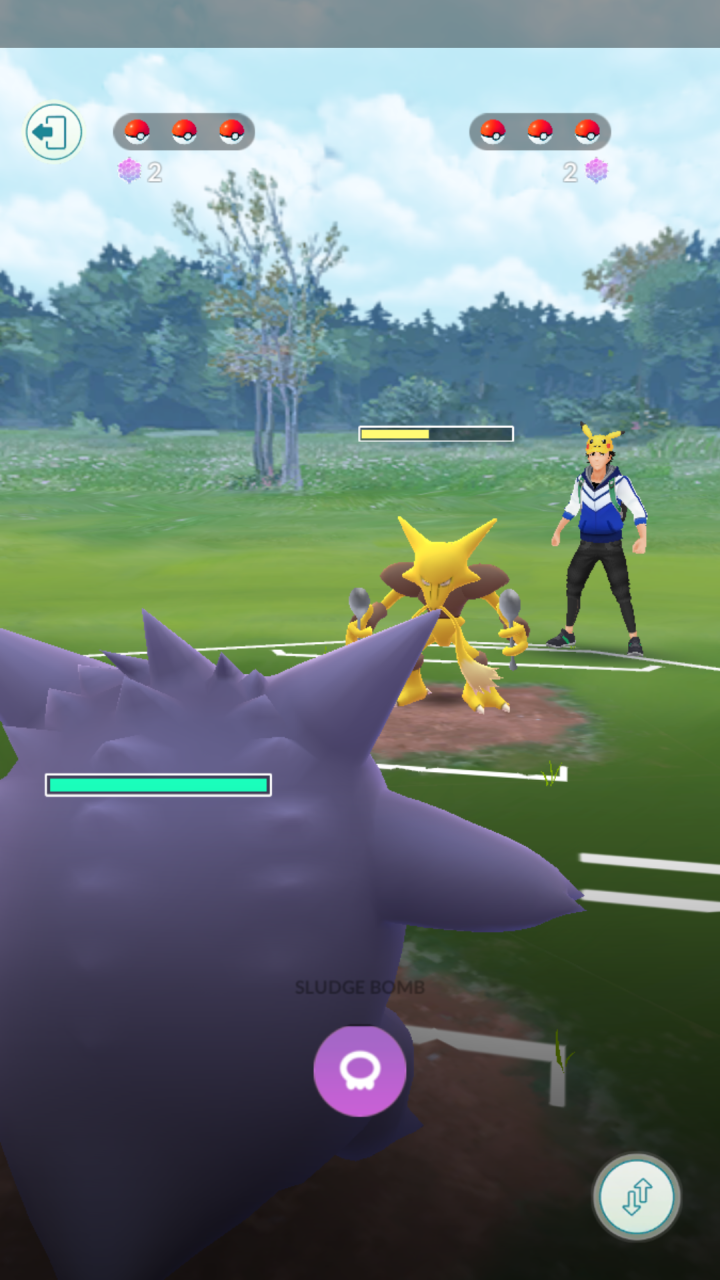
\includegraphics[scale=0.5]{slike/Slika2.2.PNG} %veličina u odnosu na širinu linije
			\centering
			\caption{Primjer borbe u Pokemon GO}
			\label{fig:promjene2} %label mora biti drugaciji za svaku sliku
		\end{figure}
		
		
		\eject
		
	
\chapter{Specifikacija programske potpore}

\section{Funkcionalni zahtjevi}

\textbf{\textit{dio 1. revizije}}\\

%\textit{Navesti \textbf{dionike} koji imaju \textbf{interes u ovom sustavu} ili  \textbf{su nositelji odgovornosti}. To su prije svega korisnici, ali i administratori sustava, naručitelji, razvojni tim.}\\

%\textit{Navesti \textbf{aktore} koji izravno \textbf{koriste} ili \textbf{komuniciraju sa sustavom}. Oni mogu imati inicijatorsku ulogu, tj. započinju određene procese u sustavu ili samo sudioničku ulogu, tj. obavljaju određeni posao. Za svakog aktora navesti funkcionalne zahtjeve koji se na njega odnose.}\\


\noindent \textbf{Dionici:}

\begin{packed_enum}
	
	\item Administrator
	\item Kartograf			
	\item Igrač/korisnik	
	\item Neregistrirani/neprijavljeni korisnik
	\item Baza podataka - U primjeru dokumentacije nije navedena
	\item Razvojni tim
	
	
\end{packed_enum}

\noindent \textbf{Aktori i njihovi funkcionalni zahtjevi:}


\begin{packed_enum}
	\item  \underbar{Neregistrirani/neprijavljeni korisnik(inicijator) može se:}
	
	\begin{packed_enum}
		
		\item registrirati u sustav, stvoriti novi korisnički račun za koji su mu potrebni korisničko ime,
		fotografija, lozinka, email adresa i lokacija uređaja.
		\begin{packed_enum}
			
			\item  ukoliko se korisnik želi registrirati kao kartograf potrebno je dodati IBAN i fotografiju osobne
			
		\end{packed_enum}
		
	\end{packed_enum}
	
	\item  \underbar{Igrač (inicijator) može:}
	
	\begin{packed_enum}
		
		\item pregledati profil drugih igrača(ime, sakupljene karte, rang, winrate, statistiku zadnih 10 borbi)
		
		\item mijenjati i pregledati svoje osobne podatke 
		
		\item sakupiti kartu ulaskom u određeni radijus stvarne lokacije
		
		\item pregledati ostale igrače unutar 50km
		\begin{packed_enum}
			
			\item moguće poslati zahtjev za borbu dostupnim igračima
			
		\end{packed_enum}
		
		\item pregledati stvarnu mapu i svoju poziciju ---  \textit{google-ova ili slično} 
		
		\item pregledati naziv, opis, fotografiju i jačinu karte iz preglednika stvarne mape(pop out)
		
		\item prijaviti željenu lokaciju u blizini i ispuniti atribute
		
		\item pregledati globalnu statistiku odigranih borbi
		
		\item pregledati globalnu statistiku sakupljenih karata
		
		\item pregledati elo poredak svih igrača
		
		\item birati karte za špil koji se koristi u borbama
		
		
	\end{packed_enum}
	\item  \underbar{Kartograf (inicijator) može:}
	
	\begin{packed_enum}
		
		\item pregledati sve prijavljene lokacije
		
		\item potvrditi, odbiti i urediti prijavljene lokacije
		\begin{packed_enum}
			
			\item označiti prijavljenu lokaciju za potvrdu s terena
			
		\end{packed_enum}
		
		\item odabrati koje će lokacije potvrditi s terena
		
	\end{packed_enum}
	
	\item  \underbar{Administrator (inicijator) može:}
	
	\begin{packed_enum}
		
		\item sve funkcionalnosti igrača i kartografa
		
		\item potvrditi registraciju kartografa
		
		\item privremeno isključiti igrača iz igre
		
		\item urediti postojeće lokacije(karte) u igri
		
		\item vidjeti i uređivati popis svih korisnika i njihovih osobnih podataka. 
		
	\end{packed_enum}
	
	\item  \underbar{Baza podataka (sudionik): }
	
	\begin{packed_enum}
		
		\item pohranjuje sve podatke o korisnicima i njihovim ovlastima
		
		\item pohranjuje sve podatke o lokacijama (kartama)
		
		\item  pohranjuje podatke o borbama
		
		
	\end{packed_enum}
\end{packed_enum}

\eject 



\subsection{Obrasci uporabe}

\textbf{\textit{dio 1. revizije}}

\subsubsection{Opis obrazaca uporabe}
%\textit{Funkcionalne zahtjeve razraditi u obliku obrazaca uporabe. Svaki obrazac je potrebno razraditi prema donjem predlošku. Ukoliko u nekom koraku može doći do odstupanja, potrebno je to odstupanje opisati i po mogućnosti ponuditi rješenje kojim bi se tijek obrasca vratio na osnovni tijek.}\\

\noindent \underbar{\textbf{UC1 -  Registracija kao igrač ili kao kartograf}}
\begin{packed_item}
	\item \textbf{Glavni sudionik: } Igrač, Kartograf
	\item  \textbf{Cilj:} Stvoriti korisnički račun za pristup
	\item  \textbf{Sudionici:} Baza podataka
    \item \textbf{Preduvjeti:} 
    \item[] \begin{packed_enum}
        \item Korisnik prijavljen kao igrač ili administrator
    \end{packed_enum}
	\item  \textbf{Opis osnovnog tijeka:}
	\item[] \begin{packed_enum}
	\item Odabir načina registriranja
	\item Unos korisničkih podataka u svrhu registracije
    \item Pop Up obavijest o uspješnoj registraciji
	\end{packed_enum}
	\item  \textbf{Opis mogućih odstupanja:}
	\item[] \begin{packed_enum}
	    \item Odabir već zauzetog profilnog imena i/ili e-maila. Unos neispravnog formata ili nepostojeće e-mail adrese.
        \item[] \begin{packed_enum}
        	\item Sustav obavještava korisnika o neuspjelom upisu i vraća ga na neispunjenu formu registracije za ponovni pokušaj.
            \item Korisnik mijenja potrebne podatke te uspijeva u registaciji ili od nje odustaje.
        \end{packed_enum}
	\end{packed_enum}
\end{packed_item}

\noindent \underbar{\textbf{UC2 -  Sakupljanje karata}}
\begin{packed_item}
	\item \textbf{Glavni sudionik: } Igrač ili administrator
	\item  \textbf{Cilj:} Skupljanje nove igraće karte s određene lokacije
	\item  \textbf{Sudionici:} Baza podataka
    \item \textbf{Preduvjeti:}
	\item[]  \begin{packed_enum}
	    \item Korisnik prijavljen kao igrač ili administrator
        \item Broj karata koju igrač posjeduje je manja od gornjeg limita
        \item Korisnik se nalazi na lokaciji te karte
	\end{packed_enum}
	\item  \textbf{Opis osnovnog tijeka:}
	\item[] \begin{packed_enum}
        \item Korisnik dođe do lokacije karte
        \item Korisnik odabire "Skupi kartu lokacije"
		\item Aplikacija dodjeljuje korisniku kartu
	\end{packed_enum}
	\item  \textbf{Opis mogućih odstupanja:}
	\item[] \begin{packed_enum}
	    \item Broj karata u posjedu igrača je već dosegnuo gornji limit
        \item[] \begin{packed_enum}
        	\item Sustav obavještava korisnika o neuspjelom prihvaćanju karte i vraća ga na kartu početnog zaslona
        \end{packed_enum}
	\end{packed_enum}
\end{packed_item}

\noindent \underbar{\textbf{UC3 -  Korisnik ulazi u borbu sa drugim korisnicima}}
\begin{packed_item}
	\item \textbf{Glavni sudionik:} Igrač ili administrator
	\item  \textbf{Cilj:} Borba između igrača s ciljem osvajanja ELO bodova
	\item  \textbf{Sudionici:} Baza podataka
    \item \textbf{Preduvjeti:}
	\item[]  \begin{packed_enum}
	    \item Korisnici su prijavljeni kao igrač ili administrator
        \item Drugi korisnik je udaljen od prvog do 50 km
        \item Drugi korisnik je u tom trenutku također aktivan
	\end{packed_enum}
	\item  \textbf{Opis osnovnog tijeka:}
	\item[] \begin{packed_enum}
        \item Korisniku se prikazuju profili igrača u blizini
        \item Korisnik odabire "Profil" nekog igrača
        \item Aplikacija prikazuje profil drugog igrača
        \item Korisnik odabire "Izazovi"
        \item Drugi korisnik prihvaća izazov i korisnici ulaze u borbu jedan protiv drugoga
        \item Igrač odabire kartu koju bi htio odigrati
        \item Računalo evaulira pobjednika borbe znajući jačine odigranih karata i zapisuje rezultat u bazu podataka
        \item Korisniku se prikazuje konačan ishod borbe
        \item Karti s kojom je korisnik igrao se smanjuje vrijednost
	\end{packed_enum}
	\item  \textbf{Opis mogućih odstupanja:} 
    \item[] \begin{packed_enum}
        \item Drugi korisnik je bio unutar 50 km ali je izašao u međuvremenu dok ga je korisnik pozvao na borbu
        \item Drugi korisnik je odbio izazov
    \end{packed_enum}
\end{packed_item}

\noindent \underbar{\textbf{UC4 -  Igrač može vidjeti naziv, fotografiju, opis i jačinu karte}}
\begin{packed_item}
	\item \textbf{Glavni sudionik: } Igrač ili administrator
	\item  \textbf{Cilj:} Informiranje korisnika o određenoj igračoj karti
	\item  \textbf{Sudionici:} Baza podataka
    \item \textbf{Preduvjeti:} Korisnik je prijavljen kao igrač ili administrator
	\item  \textbf{Opis osnovnog tijeka:} 
    \item[] \begin{packed_enum}
        \item Klikom miša korisnik ulazi u kartu
        \item Korisniku se prikazuje karta
    \end{packed_enum}
\end{packed_item}

\noindent \underbar{\textbf{UC5 - Prijavljivanje željene lokacije}}
\begin{packed_item}
	\item \textbf{Glavni sudionik: } Igrač ili administrator
	\item  \textbf{Cilj:} Dodati lokaciju
	\item  \textbf{Sudionici:} Baza podataka
    \item \textbf{Preduvjeti:}
	\item[]  \begin{packed_enum}
	    \item Korisnik je registriran kao igrač ili administrator
        \item Korisnik treba biti u blizini željene lokacije
        \item Igrač treba imati sakupljeno dovoljno iskustva 
	\end{packed_enum}
	\item  \textbf{Opis osnovnog tijeka:}
	\item[] \begin{packed_enum}
	\item Korisnik odabire opciju "Predloži lokaciju"
	\item Korisnik ispunjava podatke o lokaciji
	\end{packed_enum}
	\item  \textbf{Opis mogućih odstupanja:}
	\item[] \begin{packed_enum}
	    \item Korisnik predlaže lokaciju koja je već na karti označena 
	\end{packed_enum}
\end{packed_item}

\noindent \underbar{\textbf{UC6 - Pregled profila igrača}}
\begin{packed_item}
    \item \textbf{Glavni sudionik: }Igrač ili administrator
    \item \textbf{Cilj: }Pregledati profil bilo kojeg igrača
    \item \textbf{Sudionici: }Baza podataka
    \item \textbf{Preduvjet: }Korisnik registriran kao igrač ili administrator
    \item \textbf{Opis osnovnog tijeka: }
    \item[] \begin{packed_enum}
        \item Korisnik odabire profil igrača
        \item Prikazuje se profil igrača
    \end{packed_enum}
\end{packed_item}

\noindent \underbar{\textbf{UC7 - Prikaz sakupljenih karata igrača na profilu}}
\begin{packed_item}
    \item \textbf{Glavni sudionik: }Igrač ili administrator
    \item \textbf{Cilj: } Prikazati sakupljene karte igrača
    \item \textbf{Sudionici: }Baza podataka
    \item \textbf{Preduvjet: }Korisnik je registriran kao igrač ili administrator
    \item \textbf{Opis osnovnog tijeka: }
    \item[] \begin{packed_enum}
        \item Korisnik odabire profil igrača
        \item Prikazuju se sve sakupljene karte odabranog igrača 
    \end{packed_enum}
\end{packed_item}

\noindent \underbar{\textbf{UC8 - Prikaz ranga igrača na profilu}}
\begin{packed_item}
    \item \textbf{Glavni sudionik: }Igrač ili administrator
    \item \textbf{Cilj: }Pregledati rang bilo kojeg igrača
    \item \textbf{Sudionik: }Baza podataka
    \item \textbf{Preduvjet: }Korisnik je registriran kao igrač ili administrator
    \item \textbf{Opis osnovnog tijeka:}
    \item[] \begin{packed_enum}
        \item Korisnik odabire profil igrača 
        \item Prikazuje se rang odabranog igrača
    \end{packed_enum}
\end{packed_item}

\noindent \underbar{\textbf{UC9 - Prikaz statistike zadnjih 10 borbi igrača na profilu}}
\begin{packed_item}
    \item \textbf{Glavni sudionik: }Igrač ili administator
    \item \textbf{Cilj: } Pregledati zadnjih 10 borbi i njihov rezultat
    \item \textbf{Sudionici: }Baza podataka
    \item \textbf{Preduvjet: }Korisnik je registriran kao igrač ili administrator
    \item \textbf{Opis osnovnog tijeka: }
    \item[] \begin{packed_enum}
        \item Korisnik odabire profil igrača
        \item Prikazuje se zadnjih 10 borbi i njihov rezultat
    \end{packed_enum}
\end{packed_item}

\noindent \underbar{\textbf{UC10 - Prikaz globalne statistike odigranih borbi svih igrača}}
\begin{packed_item}
    \item \textbf{Glavni sudionik: }Igrač ili administrator
    \item \textbf{Cilj: }Pregledati globalnu statistiku borbi svih igrača
    \item \textbf{Sudionici: }Baza podataka
    \item \textbf{Preduvjet: }Korisnik je prijavljen kao igrač ili administrator
    \item \textbf{Opis osnovnog tijeka: }
    \item[] \begin{packed_enum}
        \item Korisnik odabire "Globalna statistika borbi"
        \item Prikazuje se globalna statistika svih odigranih borbi
    \end{packed_enum}
\end{packed_item}

\noindent \underbar{\textbf{UC11 - Prikaz globalne statistike svih lokacija}}
\begin{packed_item}
    \item \textbf{Glavni sudionik: }Igrač ili administrator
    \item \textbf{Cilj: }Pregledati globalnu statistiku lokacija
    \item \textbf{Sudionici: }Baza podataka
    \item \textbf{Preduvjet: }Korisnik je prijavljen kao igrač ili administrator
    \item \textbf{Opis osnovnog tijeka: }
    \item[] \begin{packed_enum}
        \item Korisnik odabire "Sve lokacije"
        \item Prikazuje se sve lokacije koje se nalaze u igrici
    \end{packed_enum}
\end{packed_item}

\noindent \underbar{\textbf{UC12 – Pregled poretka igrača}}
\begin{packed_item}
	
	\item \textbf{Glavni sudionik: }Igrač, Administrator
	\item  \textbf{Cilj:} Pregledati poretke svih igrača
	\item  \textbf{Sudionici:} Baza podataka
	\item  \textbf{Preduvjet:} Korisnik je već prijavljen kao igrač ili administrator
	\item  \textbf{Opis osnovnog tijeka:}
	
	\item[] \begin{packed_enum}
		
		\item Korisnik odabire opciju „Poredak igrača“
		\item Prikaže se trenutni poredak svih igrača koji je izračunat prema elo sustavu
	\end{packed_enum}
\end{packed_item}

\noindent \underbar{\textbf{UC13 – Pregled prijavljenih lokacija}}
\begin{packed_item}
	
	\item \textbf{Glavni sudionik: }Kartograf, Administrator
	\item  \textbf{Cilj:} Pregledati sve lokacije koje su igrači prijavili
	\item  \textbf{Sudionici:} Baza podataka
	\item  \textbf{Preduvjet:} Korisnik je već prijavljen kao kartograf ili administrator
	\item  \textbf{Opis osnovnog tijeka:}
	
	\item[] \begin{packed_enum}
		
		\item Korisnik u aplikaciji odabire opciju „Pregled prijavljenih lokacija“
		\item Prikaže se karta na kojoj su označene sve lokacije koje su igrači prijavili
		\item Korisnik klikne na jednu od lokacija na karti
		\item Prikazuju se podatci o lokaciji te tri opcije (potvrdi, uredi i obriši)
	\end{packed_enum}
\end{packed_item}

\noindent \underbar{\textbf{UC14 – Potvrđivanje prijavljenih lokacija}}
\begin{packed_item}
	
	\item \textbf{Glavni sudionik: }Kartograf, Administrator
	\item  \textbf{Cilj:} Prihvatiti prijavljenu lokaciju
	\item  \textbf{Sudionici:} Baza podataka
	\item  \textbf{Preduvjet:} Korisnik je već prijavljen kao kartograf ili administrator
	\item  \textbf{Opis osnovnog tijeka:}
	
	\item[] \begin{packed_enum}
		
		\item Korisnik u aplikaciji odabire opciju „Pregled prijavljenih lokacija“
		\item Prikaže se karta na kojoj su označene sve lokacije koje su igrači prijavili
		\item Korisnik klikne na jednu od lokacija na karti
		\item Korisnik odabire opciju "Potvrdi"
		\item Lokacija se u bazi podataka označuje kao potvrđena
		\item Lokacija postaje vidljiva igračima unutar aplikacije
		\item Igrač koji je prijavio lokaciju dobiva potvrđenu kartu
	\end{packed_enum}
	
	\item  \textbf{Opis mogućih odstupanja:}
	
	\item[] \begin{packed_item}
		
		\item[3.a]  U bazi nema prijavljenih lokacija
		
	\end{packed_item}
\end{packed_item}

\noindent \underbar{\textbf{UC15 – Uređivanje prijavljenih lokacija}}
\begin{packed_item}
	
	\item \textbf{Glavni sudionik: }Kartograf, Administrator
	\item  \textbf{Cilj:} Urediti prijavljenu lokaciju
	\item  \textbf{Sudionici:} Baza podataka
	\item  \textbf{Preduvjet:} Korisnik je već prijavljen kao kartograf ili administrator
	\item  \textbf{Opis osnovnog tijeka:}
	
	\item[] \begin{packed_enum}
		
		\item Korisnik u aplikaciji odabire opciju „Pregled prijavljenih lokacija“
		\item Prikaže se karta na kojoj su označene sve lokacije koje su igrači prijavili
		\item Korisnik klikne na jednu od lokacija na karti
		\item Korisnik odabire opciju "Uredi"
		\item Korisnik mijenja podatke o lokaciji
		\item Korisnik klikne na gumb "Spremi promjene"
		\item Baza podataka se ažurira
	\end{packed_enum}
	
	\item  \textbf{Opis mogućih odstupanja:}
	
	\item[] \begin{packed_item}
		
		\item[3.a]  U bazi nema prijavljenih lokacija
		\item[5.a]  Korisnik nije spremio podatke
		\item[] \begin{packed_enum}
			
			\item Sustav obavještava korisnika da nije spremio podatke
			
		\end{packed_enum}
		
	\end{packed_item}
\end{packed_item}

\noindent \underbar{\textbf{UC16 – Odbijanje prijavljenih lokacija}}
\begin{packed_item}
	
	\item \textbf{Glavni sudionik: }Kartograf, Administrator
	\item  \textbf{Cilj:} Odbiti prijavljenu lokaciju
	\item  \textbf{Sudionici:} Baza podataka
	\item  \textbf{Preduvjet:} Korisnik je već prijavljen kao kartograf ili administrator
	\item  \textbf{Opis osnovnog tijeka:}
	
	\item[] \begin{packed_enum}
		
		\item Korisnik u aplikaciji odabire opciju „Pregled prijavljenih lokacija“
		\item Prikaže se karta na kojoj su označene sve lokacije koje su igrači prijavili
		\item Korisnik klikne na jednu od lokacija na karti
		\item Korisnik odabire opciju "Obriši"
		\item Lokacija se uklanja iz baze podataka
	\end{packed_enum}
	
	\item  \textbf{Opis mogućih odstupanja:}
	
	\item[] \begin{packed_item}
		
		\item[3.a]  U bazi nema prijavljenih lokacija
		
	\end{packed_item}
\end{packed_item}

\noindent \underbar{\textbf{UC17 -Pregled lokacija kojima je potrebna potvrda s terena}}
\begin{packed_item}
	
	\item \textbf{Glavni sudionik: }Kartograf, Administrator
	\item  \textbf{Cilj:} Pregled svih lokacija kojima je potrebna potvrda s terena
	\item  \textbf{Sudionici:} Baza podataka
	\item  \textbf{Preduvjet:} Korisnik je prijavljen kao kartograf ili administrator
	\item  \textbf{Opis osnovnog tijeka:}
	
	\item[] \begin{packed_enum}
		
		\item Korisnik odabire opciju "Pregled lokacija za potvrdu s terena"
		\item Prikaže se lista lokacija koje zahtijevaju potvrdu s terena
	\end{packed_enum}
\end{packed_item}


\noindent \underbar{\textbf{UC18 - Odabiranje lokacija za osobnu potvrdu s terena}}
\begin{packed_item}
	
	\item \textbf{Glavni sudionik: }Kartograf, Administrator
	\item  \textbf{Cilj:} Označiti koje od lokacija za potvrdu s terena će korisnik osobno provjeriti
	\item  \textbf{Sudionici:} Baza podataka
	\item  \textbf{Preduvjet:} Korisnik je prijavljen kao kartograf ili administrator
	\item  \textbf{Opis osnovnog tijeka:}
	
	\item[] \begin{packed_enum}
		
		\item Korisnik odabire opciju "Pregled lokacija za potvrdu s terena"
		\item Prikaže se lista lokacija koje zahtjevaju potvrdu s terena
		\item Korisnik označava lokacije koje on želi osobno provjeriti
		\item Nakon pritiska gumba "Dohvati put", označene lokacije postanu vidljive samo tom korisniku na stranici "Pregled lokacija za potvrdu s terena"
		\item Sustav preko vanjskog servisa OSRM dohvati rješenje problema trgovačkog putnika
		\item Sustav korisniku put prikaže na karti na stranici „Pregled prijavljenih lokacija“
		\item Korisnik je preusmjeren na stranicu „Pregled prijavljenih lokacija“
	\end{packed_enum}	
	
	\item  \textbf{Opis mogućih odstupanja:}
	
	\item[] \begin{packed_item}
		
		\item[3.a] Korisnik nikad ne potvrdi lokaciju s terena
		\item[] \begin{packed_enum}
			
			\item Postaviti vremenski rok od trenutka prihvaćanja
			
		\end{packed_enum}
		\item[4.a] Korisnik ne pritisne gumb "Dohvati put" te pokuša izaći iz stranice
		\item[] \begin{packed_enum}
			
			\item Sustav obaviještava korisnika da nije spremio podatke
			
		\end{packed_enum}
		\item[4.b] Korisnik je imao prethodno označene lokacije
		\item[] \begin{packed_enum}
			
			\item Lokacije koje više nisu označene su ponovno vidljive svim korisnicima
			
		\end{packed_enum}
	\end{packed_item}
\end{packed_item}


\noindent \underbar{\textbf{UC19 -Potvrda registracije kartografa}}
\begin{packed_item}
	
	\item \textbf{Glavni sudionik: } Administrator
	\item  \textbf{Cilj:} Prihvatiti kartografa u sustav
	\item  \textbf{Sudionici:} Kartograf, Baza podataka
	\item  \textbf{Preduvjet:} Korisnik je registriran i dodijeljena su mu prava administratora
	\item  \textbf{Opis osnovnog tijeka:}
	
	\item[] \begin{packed_enum}
		
		\item Administrator odabire opciju "Pregled prijavljenih kartografa"
		\item Prikaže se lista prijavljenih kartografa s opcijama "Potvrdi" i "Odbij" pored svakog kartografa
		\item Administrator klikne na gumb "Potvrdi"
		\item Kartograf se sprema u bazu kao potvrđen
	\end{packed_enum}
\end{packed_item}

\noindent \underbar{\textbf{UC20 -Odbijanje registracije kartografa}}
\begin{packed_item}
	
	\item \textbf{Glavni sudionik: } Administrator
	\item  \textbf{Cilj:} Odbiti prijavu kartografa
	\item  \textbf{Sudionici:} Kartograf, Baza podataka
	\item  \textbf{Preduvjet:} Korisnik je registriran i dodijeljena su mu prava administratora
	\item  \textbf{Opis osnovnog tijeka:}
	
	\item[] \begin{packed_enum}
		
		\item Administrator odabire opciju "Pregled prijavljenih kartografa"
		\item Prikaže se lista prijavljenih kartografa s opcijama "Potvrdi" i "Odbij" pored svakog kartografa
		\item Administrator klikne na gumb "Odbij"
		\item Kartograf se briše iz baze podataka
	\end{packed_enum}
\end{packed_item}

\noindent \underbar{\textbf{UC21 - Prikazivanje popisa igrača u blizini}}
\begin{packed_item}
	
	\item \textbf{Glavni sudionik: } Igrač ili Administrator
	\item \textbf{Cilj:} Pregledati korisnike u blizini kao potencijalne suparnike za borbu
	\item \textbf{Sudionici:} Baza podataka
	\item \textbf{Preduvjet:} 
    \item[] \begin{packed_enum}
        \item Korisnik je prijavljen kao igrač ili administrator
        \item Drugi korisnik je udaljen od prvog do 50 km
        \item Drugi korisnik je u tom trenutku također aktivan    
    \end{packed_enum}
	\item  \textbf{Opis osnovnog tijeka:}
	\item[] \begin{packed_enum}
        \item Korisnik odabire opciju "Igrači u blizini"
        \item Korisniku se prikazuje lista profila ostalih korisnika u blizini
	\end{packed_enum}
\end{packed_item}

\noindent \underbar{\textbf{UC22 -Privremeno isključivanje igrača iz igre}}
\begin{packed_item}
	
	\item \textbf{Glavni sudionik: }Administrator
	\item  \textbf{Cilj:} Privremeno onemogućiti igraču igru
	\item  \textbf{Sudionici:} Igrač, Baza podataka
	\item  \textbf{Preduvjet:} Korisnik je registriran i dodijeljena su mu prava administratora
	\item  \textbf{Opis osnovnog tijeka:}
	
	\item[] \begin{packed_enum}
		
		\item Administrator odabire opciju "Pregled svih korisnika"
		\item Prikaže se lista svih korisnika
		\item Administrator odabire igača kojeg želi isključiti te pritisne gumb "Ban" pored njegovog imena
		\item Baza podataka se ažurira te odabran igrač postaje suspendiran na 30 dana
		
	\end{packed_enum}
\end{packed_item}


\noindent \underbar{\textbf{UC23 - Uređivanje postojećih lokacija u igri}}
\begin{packed_item}
	\item \textbf{Glavni sudionik: }Administrator
	\item  \textbf{Cilj:} Urediti prethodno potvrđenu lokaciju
	\item  \textbf{Sudionici:} Baza podataka
	\item  \textbf{Preduvjet:}Korisnik je registriran i dodijeljena su mu prava administratora
	\item  \textbf{Opis osnovnog tijeka:}
	\item[] \begin{packed_enum}
		\item Administrator odabire opciju "Pregled svih lokacija"
		\item Prikaže se lista svih lokacija koje je prethodno potvrdio kartograf ili administrator
		\item Administrator odabire lokaciju čije podatke želi izmjeniti
		\item Popunjava obrazac novim podacima i stisne gumb "Primijeni"
		\item Baza podataka se ažurira
	\end{packed_enum}
	\item  \textbf{Opis mogućih odstupanja:}
	\item[] \begin{packed_enum}
		\item Neko od polja obrasca nije ispravno popunjeno u trenutku podnošenja obrasca
		\item[] \begin{packed_enum}
			\item Sustav obavještava administratora o neuspjeloj promijeni podataka
		\end{packed_enum}
	\end{packed_enum}
\end{packed_item}


\subsubsection{Dijagrami obrazaca uporabe}

		%unos slike
		\begin{figure}[H]
			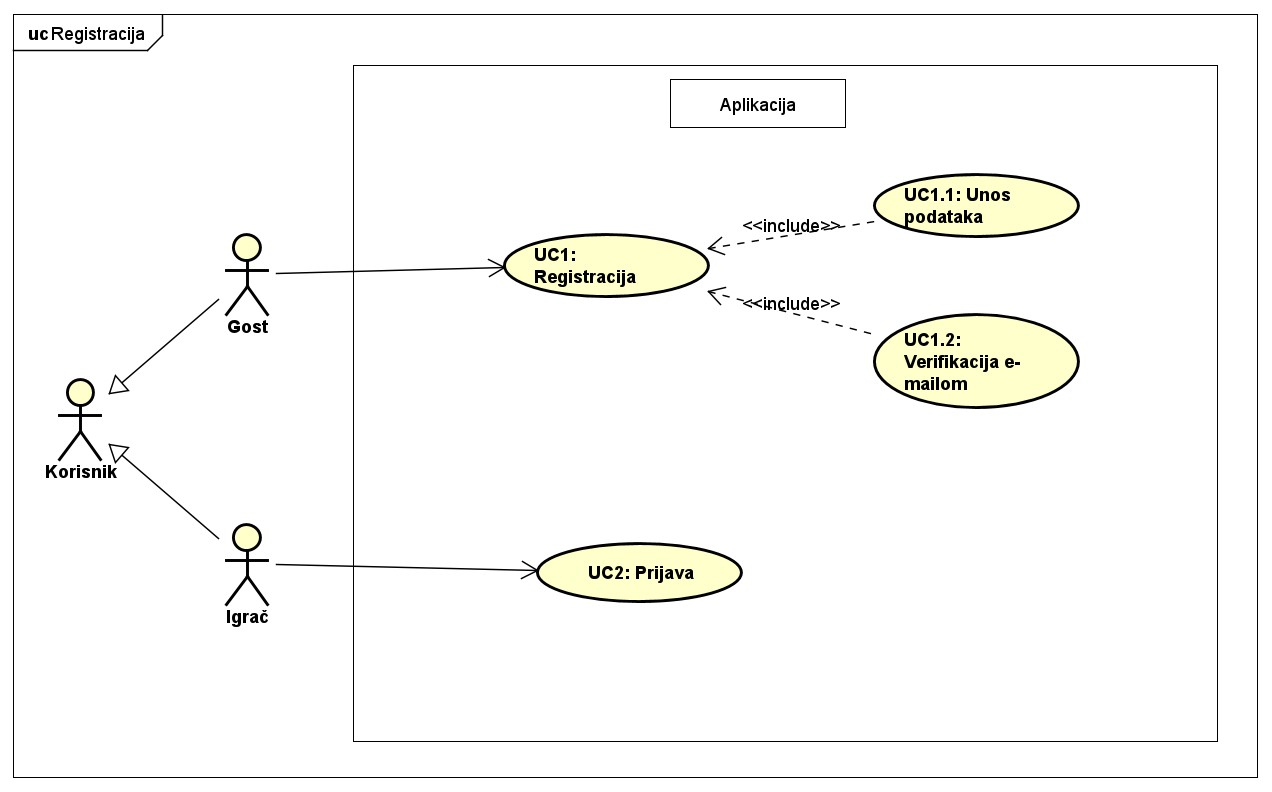
\includegraphics[width=\textwidth]{slike/UCRegistracija.png} %veličina u odnosu na širinu linije
			\caption{Prikaz UC za registraciju i prijavu}
			\label{fig:UCregistracija} %label mora biti drugaciji za svaku sliku
		\end{figure}
\pagebreak

		%unos slike
		\begin{figure}[H]
			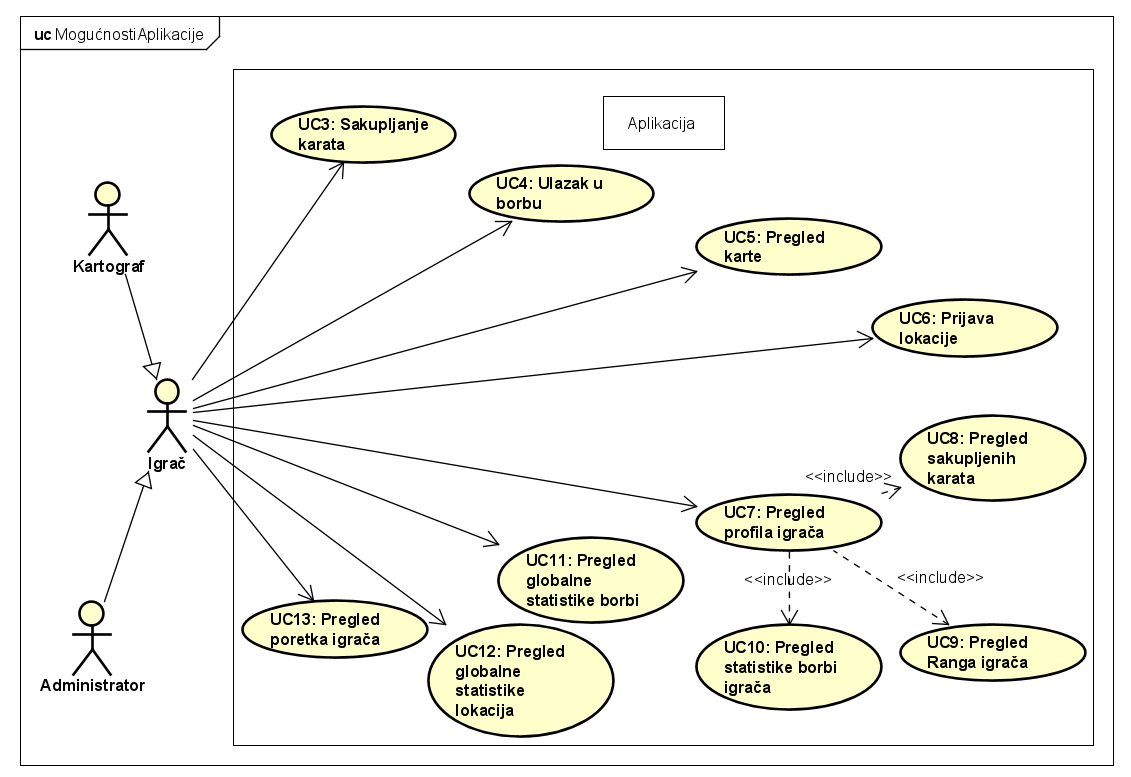
\includegraphics[width=\textwidth]{slike/UCMogucnostiAplikacije.png} %veličina u odnosu na širinu linije
			\caption{Prikaz UC za osnovne mogućnosti aplikacije dostupne igračima}
			\label{fig:UCmogucnostiAplikacije} %label mora biti drugaciji za svaku sliku
		\end{figure}
\pagebreak

		%unos slike
		\begin{figure}[H]
			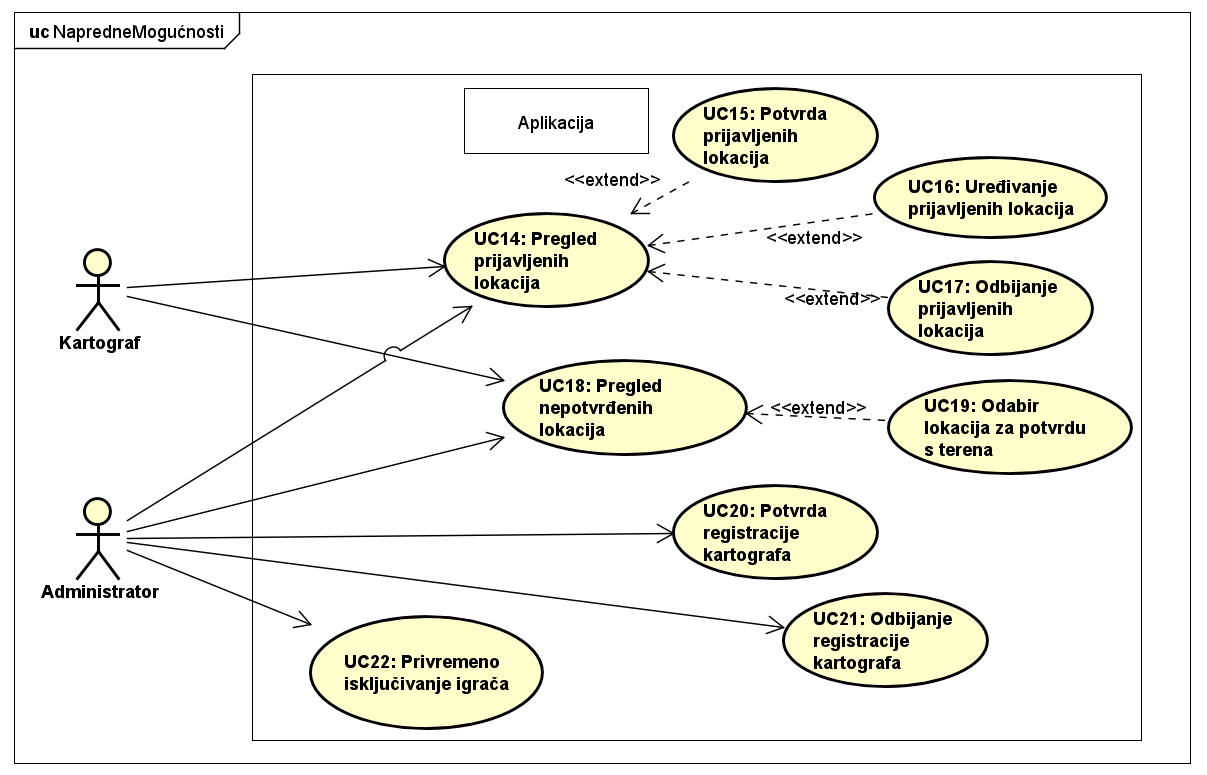
\includegraphics[width=\textwidth]{slike/UCNapredneMogucnosti.png} %veličina u odnosu na širinu linije
			\caption{Prikaz UC za napredne mogućnosti dostupne kartografima i administratorima}
			\label{fig:UCnapredneMogucnosti} %label mora biti drugaciji za svaku sliku
		\end{figure}
\pagebreak

%\textit{Prikazati odnos aktora i obrazaca uporabe odgovarajućim UML dijagramom. Nije nužno nacrtati sve na jednom dijagramu. Modelirati po razinama apstrakcije i skupovima srodnih funkcionalnosti.}
\eject		

\subsection{Sekvencijski dijagrami}

\textbf{\textit{dio 1. revizije}}\\

\noindent \textbf{Obrazac uporabe UC2 - Sakupljanje karata}
    Korisnik vidi na mapi kartu koju bi želio sakupiti. Korisnik odlazi do lokacije gdje može dobiti tu kartu. Dolaskom na lokaciju i odabirom "Skupi kartu lokacije" korisnik šalje zahtjev aplikaciji za sakupljanje karte. Aplikacija provjerava nalazi li se korisnik na navedenoj lokaciji, zatim dohvaća korisnikove podatke te provjerava ima li manje od 20 karata spremljenih. Ako je provjera zadovoljena, aplikacija daje šalje zahtjev bazi podataka da spremi korisniku kartu te lokacije. Konačno, aplikacija obavještava korisnika o uspješnom, odnosno neuspješnom sakupljanju karte.

		%unos slike
		\begin{figure}[H]
			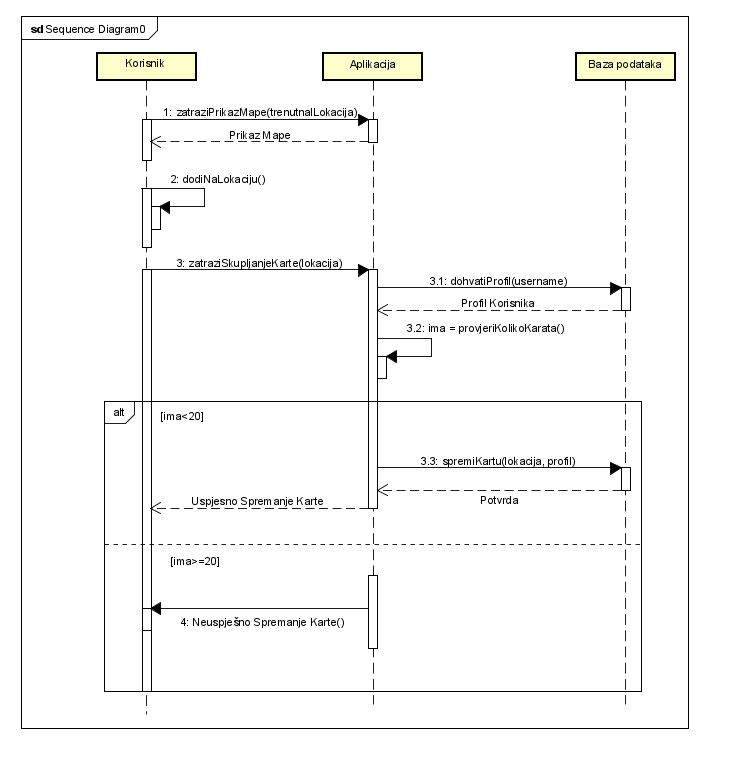
\includegraphics[width=\textwidth]{slike/SeqUC2.png} %veličina u odnosu na širinu linije
			\caption{Sekvencijski dijagram za UC2}
			\label{fig:promjene3} %label mora biti drugaciji za svaku sliku
		\end{figure}
\pagebreak

\noindent \textbf{Obrazac uporabe UC3 - Korisnik ulazi u borbu s njima}
    Korisnik želi otići u borbu. Korisnik je na stranici za prikaz ostalih korisnika u blizini. Korisnik odabire jedan profil i odabirom "Izazovi" šalje zahtjev aplikaciji za borbu protiv tog korisnika. Aplikacija šalje zahtjev drugome korisniku želi li ući u borbu s prethodnim korisnikom. Odgovor drugog korisnika aplikacija šalje natrag prvom korisniku. Ako je drugi korisnik prihvatio, aplikacija prikazuje stranicu za borbu korisnicima. Aplikacija šalje zahtjev bazi podataka za prikazom svih karata toga korisnika. Baza vraća podatke i aplikacija prikazuje korisniku njegove karte. Korisnik odabire kartu. Aplikacija uspoređuje jačinu karata i vraća rezultat korisnicima. Karti koju je korisnik koristio se smanjuje vrijednost za 10 posto. Ako drugi korisnik nije prihvatio borbu, aplikacija obaviještava korisnika o tome.
    
    		%unos slike
		\begin{figure}[H]
			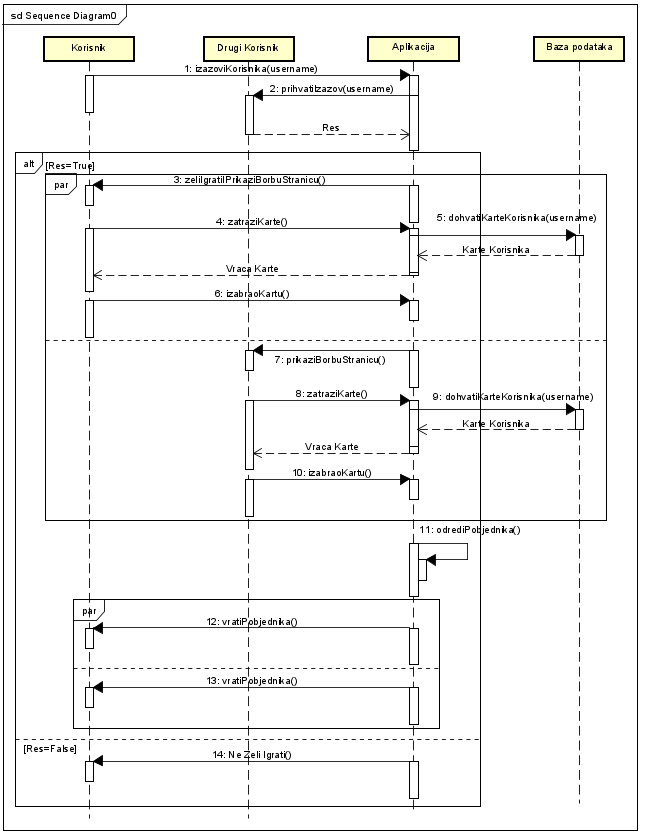
\includegraphics[width=\textwidth]{slike/SeqUC3.png} %veličina u odnosu na širinu linije
			\caption{Sekvencijski dijagram za UC3}
			\label{fig:promjene4} %label mora biti drugaciji za svaku sliku
		\end{figure}
\pagebreak

\noindent \textbf{Obrazac uporabe UC5 - Prijavljivanje željene lokacije}
    
    Korisnik se nalazi na mjestu koje je zanimljivo i želi ga dodati u aplikaciju. Korisnik odabire "Predloži lokaciju". Aplikacija dohvaća podatke o korisniku i provjerava ima li dovoljno iskustva. Ako nema dovoljno iskustva aplikacija obaviještava korisnika o tome. Ako ima dovoljno iskustva prikazuje stranicu u kojoj traži informacije o novoj lokaciji. Nakon što korisnik ispuni podatke i preda informacije, aplikacija šalje zahtjev bazi podataka da spremi navedenu lokaciju. Tu lokaciju baza sprema kao nepotvrđenu. Uz to baza sprema i podatke o korisniku koji je predložio lokaciju kako bi mu aplikacija kasnije mogla dati tu kartu.
    		%unos slike
		\begin{figure}[H]
			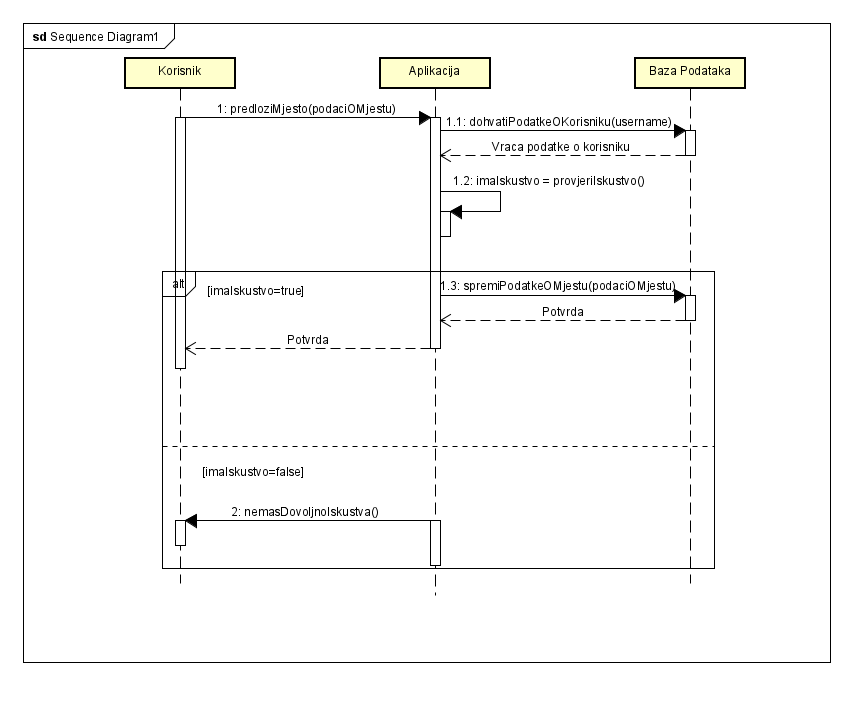
\includegraphics[width=\textwidth]{slike/SeqUC5.png} %veličina u odnosu na širinu linije
			\caption{Sekvencijski dijagram za UC3}
			\label{fig:promjene5} %label mora biti drugaciji za svaku sliku
		\end{figure}
\eject

\section{Ostali zahtjevi}

%\textbf{\textit{dio 1. revizije}}\\

%\textit{Nefunkcionalni zahtjevi i zahtjevi domene primjene dopunjuju funkcionalne zahtjeve. Oni opisuju \textbf{kako se sustav treba ponašati} i koja \textbf{ograničenja} treba poštivati (performanse, korisničko iskustvo, pouzdanost, standardi kvalitete, sigurnost...). Primjeri takvih zahtjeva u Vašem projektu mogu biti: podržani jezici korisničkog sučelja, vrijeme odziva, najveći mogući podržani broj korisnika, podržane web/mobilne platforme, razina zaštite (protokoli komunikacije, kriptiranje...)... Svaki takav zahtjev potrebno je navesti u jednoj ili dvije rečenice.}
	
		\begin{packed_item}
			\item Sustav treba omogućiti rad više korisnika u stvarnom vremenu
			\item Korisničko sučelje i sustav moraju podržavati hrvatsku abecedu (dijakritičke znakove) pri unosu i prikazu tekstualnog sadržaja
			\item Izvršavanje dijela programa u kojem se pristupa bazi podataka ne smije trajati duže od nekoliko sekundi
			\item Sustav treba biti implementiran kao web aplikacija koristeći objektno-orijentirane jezike
			\item Neispravno korištenje korisničkog sučelja ne smije narušiti funkcionalnost i rad sustava
			\item Sustav treba biti jednostavan za korištenje, korisnici se moraju znati koristiti sučeljem bez opširnih uputa
			\item Nadogradnja sustava ne smije narušavati postojeće funkcionalnosti sustava
			\item Veza s bazom podataka mora biti kvalitetno zaštićena, brza i otporna na vanjske greške
			\item Pristup sustavu mora biti omogućen iz javne mreže pomoću HTTPS
			\item Korisnik u svakom trenutku mora imati pristup GPS - u
			\item Moraju biti osigurana konzistentna prava i mogućnosti svim igračima podjednako
			\item Svaka nova registracija mora biti potvrđena putem e - mail adrese korisnika
			\item Svaka lokacija u aplikaciji mora korelirati stvarnoj lokaciji
			\item Sustav mora osigurati da svaka uloga ima samo njoj definirane ovlasti
			\item Baza podataka se kontinuirano mora osvježavati za obnovu podataka u slučaju prekida veze ili nestanka struje
		\end{packed_item}





\chapter{Arhitektura i dizajn sustava}
		
    Arhitektura sustava može se podijeliti na 3 podsustava:
    \begin{itemize}
        \item \textbf{web poslužitelj:} ključna komponenta Interneta. Njegove glavne zadaće uključuju raspoznavanje različitih URL-ova i procesuiranje HTTP zahtjeva čime se omogućuje komunikacija između klijenta i aplikacije. On pokreće web aplikaciju kojoj klijent pristupa pomoću web preglednika
        \item \textbf{web aplikacija:} program koji služi za ispunjenje klijentskih zahtjeva. Ovisno o zahtjevu, aplikacija upravlja dobivenim podacima (koje klijent šalje pomoću web preglednika), pristupa bazi podataka i vraća podatke pregledniku koji ih onda u odgovarajućem formatu prezentira klijentu
        \item \textbf{baza podataka:} služi za pohranu podataka koji se čuvaju tijekom rada te (u većini slučajeva) između različitih pristupa aplikaciji
    \end{itemize}
    
    %unos slike
		\begin{figure}[H]
			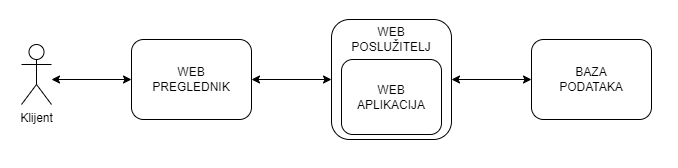
\includegraphics[scale=1]{slike/arhitektura.PNG} %veličina slike u odnosu na originalnu datoteku i pozicija slike
			\centering
			\caption{Arhitektura sustava}
			\label{fig:promjene}
		\end{figure}

	Programski jezici korišteni za razvoj aplikacije su Java zajedno sa Spring Boot radnim okvirom te JavaScript s radnim okvirom React. Arhitektura sustava temelji se na 4 sloja Spring Boot radnog okvira:
		
	\begin{itemize}
	    \item \textbf{presentation layer:} sastoji se od front-end dijela aplikacije te služi za rukovanje HTTP zahtjevima. Primljeni se zahtjevi ovjeravaju i prosljeđuju business sloju s kojim presentation sloj komunicira
	    \item \textbf{business layer:} ovaj sloj služi za rukovanje poslovnom logikom aplikacije. Sadrži klase za razne usluge te izvodi autentifikaciju i verifikaciju. Osim toga, služi kao posrednik presentation i persistence sloja
	    \item \textbf{persistence layer:} ovaj se sloj bavi logikom spremanja podataka - podatke koje dobiva od business sloja pretvara u upite nad bazom podataka te ih prosljeđuje database sloju i obrnuto
	    \item \textbf{database layer:} sloj koji izvodu CRUD (Create, Read, Update, Delete) operacije nad bazom podataka
	\end{itemize}
	

		\section{Baza podataka}
			
			%\textbf{\textit{dio 1. revizije}}\\
			
			Za potrebe sustava našeg projekta koristit ćemo relacijski bazu podataka. Osnovna građa baze je relacija. Relacija je tablica koja je definirana imenom i skupom atributa. Glavni zadatak baze podataka je brza i jednostavna pohrana, izmjena i dohvat podataka za daljnju obradu.
			Baza podataka ove aplikacije sastoji se od sljedećih tablica: 
			\begin{itemize}
				\item Korisnik
				\item Karta
				\item Borba
				\item Lokacija
				\item Vrsta lokacije
				\item Lokacija za potvrdu
			\end{itemize}
		
			\subsection{Opis tablica}
			

				%\textit{Svaku tablicu je potrebno opisati po zadanom predlošku. Lijevo se nalazi točno ime varijable u bazi podataka, u sredini se nalazi tip podataka, a desno se nalazi opis varijable. Svjetlozelenom bojom označite primarni ključ. Svjetlo plavom označite strani ključ}
				
				\textbf{Korisnik:} Ovaj entitet sadrži sve važne informacije o korisniku aplikacije. Sadrži atribute: korisničko ime, lozinka, fotografija, email, razina ovlasti, iban, fotografija osobne, bodovi i isključenje. Ovaj entitet u vezi je One-to-Many s entitetom Borba preko atributa korisničko ime korisnika, u vezi je One-to-Many s entitetom Karta preko atributa korisničko ime korisnika i u vezi je One-to-Many s entitetom Lokacija za potvrdu preko atributa korisničko ime korisnika.
				\begin{longtblr}[
					label=none,
					entry=none
					]{
						width = \textwidth,
						colspec={|X[6,l]|X[6, l]|X[20, l]|}, 
						rowhead = 1,
					} %definicija širine tablice, širine stupaca, poravnanje i broja redaka naslova tablice
					\hline \SetCell[c=1]{l}{\textbf{Korisnik}}	 \\ \hline[3pt]
					\SetCell{LightGreen}Korisničko ime & VARCHAR	&  	Jedinstveni identifikator korisnika  	\\ \hline
					Lozinka	& VARCHAR &   Hash lozinke	\\ \hline 
					Fotografija & LONGBLOB &  Fotografija korisnika \\ \hline 
					Email & VARCHAR	&  	Email korisnika	\\ \hline 
					Razina ovlasti	& VARCHAR &   Razina ovlasti korisnika \\ \hline 
					IBAN	& VARCHAR &   IBAN računa za uplatu za kartografa	\\ \hline 
					Fotografija osobne	& LONGBLOB &   Fotografija osobne iskaznice kartografa	\\ \hline 
					Bodovi	& INT &   Broj bodova koje je igrač osvojio	\\ \hline 
					Isključenje	& BOOLEAN &  Oznaka je li igrač trenutno isključen iz igre	\\ \hline 
				\end{longtblr}
				
				\textbf{Borba:} Ovaj entitet sadrži sve važne informacije vezane uz borbu. Sadrži atribute: id borba, korisničko ime protivnika, pobjednik, gubitnik i korisničko ime. Ovaj entitet u vezi je Many-to-One s entitetom Korisnik preko korisničkog imena.
				\begin{longtblr}[
					label=none,
					entry=none
					]{
						width = \textwidth,
						colspec={|X[6,l]|X[6, l]|X[20, l]|}, 
						rowhead = 1,
					} %definicija širine tablice, širine stupaca, poravnanje i broja redaka naslova tablice
					\hline \SetCell[c=1]{l}{\textbf{Borba}}	 \\ \hline[3pt]
					\SetCell{LightGreen}ID Borba & INT	&  	Jedinstveni identifikator borbe	\\ \hline
					Korisničko ime protivnika	& VARCHAR &   Korisničko ime protivnika u borbi	\\ \hline 
					Pobjednik	& VARCHAR &   Korisničko ime pobjednika u borbi	\\ \hline 
					Gubitnik	& VARCHAR &   Korisničko ime gubitnika u borbi	\\ \hline  
					\SetCell{LightBlue} Korisničko ime	& VARCHAR &   Korisničko ime korisnika koji je započeo borbu, (korisnik.korisnicko ime) 	\\ \hline 
				\end{longtblr}
			
				\textbf{Karta:} Ovaj entitet sadrži sve važne informacije vezane uz karte. Sadrži atribute: id karta, jačina karte, korisničko ime i id lokacija. Ovaj entitet u vezi je Many-to-One s entitetom Korisnik preko korisničkog imena i u vezi Many-to-one s entitetom Lokacija preko id lokacija.
				\begin{longtblr}[
					label=none,
					entry=none
					]{
						width = \textwidth,
						colspec={|X[6,l]|X[6, l]|X[20, l]|}, 
						rowhead = 1,
					} %definicija širine tablice, širine stupaca, poravnanje i broja redaka naslova tablice
					\hline \SetCell[c=1]{l}{\textbf{Karta}}	 \\ \hline[3pt]
					\SetCell{LightGreen}ID Karta & INT	&  	Jedinstveni identifikator karte	\\ \hline
					Jačina karte	& INT &   Jačina karte	\\ \hline 
					\SetCell{LightBlue} Korisničko Ime	& VARCHAR &   Jedinstveni identifikator korisnika kome pripada karta, (korisnik.korisnicko ime) 	\\ \hline
					\SetCell{LightBlue} ID Lokacija	& INT &   Jedinstveni identifikator lokacije, (lokacija.id lokacija)	\\ \hline 
				\end{longtblr}
			
				\textbf{Lokacija:} Ovaj entitet sadrži sve važne informacije vezane uz potvrđene lokacije. Sadrži atribute: id lokacije, naziv, opis, fotografija, jačina i id vrste lokacije. Ovaj entitet u vezi je Many-to-One s entitetom Vrsta lokacije preko id vrsta lokacije i One-to-Many s entitetom Karta preko id lokacija.
				\begin{longtblr}[
					label=none,
					entry=none
					]{
						width = \textwidth,
						colspec={|X[6,l]|X[6, l]|X[20, l]|}, 
						rowhead = 1,
					} %definicija širine tablice, širine stupaca, poravnanje i broja redaka naslova tablice
					\hline \SetCell[c=1]{l}{\textbf{Lokacija}}	 \\ \hline[3pt]
					\SetCell{LightGreen}ID Lokacije & INT	&  	Jedinstveni identifikator lokacije	\\ \hline
					Naziv	& VARCHAR &   Naziv lokacije	\\ \hline 
					Opis & VARCHAR &  Opis lokacije \\ \hline 
					Fotografija & LONGBLOB	&  	Fotografija lokacije	\\ \hline 
					Podatak za izračun jačine & VARCHAR	&  	Podatak za izračun početne jačine karte određene lokacije (grad-broj stanovnika,..)	\\ \hline 
					\SetCell{LightBlue} ID Vrste Lokacije	& INT &   Jedinstveni identifikator vrste lokacije (vrsta lokacije.id vrsta lokacije)	\\ \hline 
				\end{longtblr}
			
				\textbf{Vrsta lokacije:} Ovaj entitet sadrži sve važne informacije vezane uz vrste lokacija. Sadrži atribute: id vrsta lokacije i tip lokacije. Ovaj entitet u vezi je One-to-Many s entitetom Lokacija preko id vrsta lokacije i u vezi One-to-Many s entitetom Lokacija za potvrdu preko id lokacija za potvrdu.
				\begin{longtblr}[
					label=none,
					entry=none
					]{
						width = \textwidth,
						colspec={|X[6,l]|X[6, l]|X[20, l]|}, 
						rowhead = 1,
					} %definicija širine tablice, širine stupaca, poravnanje i broja redaka naslova tablice
					\hline \SetCell[c=1]{l}{\textbf{Vrsta Lokacije}}	 \\ \hline[3pt]
					\SetCell{LightGreen}ID Vrste Lokacije & INT	&  	Jedinstveni identifikator vrste lokacije  	\\ \hline
					Tip lokacije	& VARCHAR &   Naziv vrste lokacije	\\ \hline  
				\end{longtblr}
			
				\textbf{Lokacija za potvrdu:} Ovaj entitet sadrži sve važne informacije vezane uz lokacije za potvrdu. Sadrži atribute: id lokacije za potvrdu, naziv, opis, fotografija, jačina, korisničko ime kartografa, id vrste lokacije i korisničko ime. Ovaj entitet u vezi je Many-to-One s entitetom Vrsta lokacije preko id vrsta lokacije i Many-to-One s entitetom Korisnik preko korisničkog imena.
				\begin{longtblr}[
					label=none,
					entry=none
					]{
						width = \textwidth,
						colspec={|X[6,l]|X[6, l]|X[20, l]|}, 
						rowhead = 1,
					} %definicija širine tablice, širine stupaca, poravnanje i broja redaka naslova tablice
					\hline \SetCell[c=1]{l}{\textbf{Lokacija za potvrdu}}	 \\ \hline[3pt]
					\SetCell{LightGreen}ID Lokacije za potvrdu & INT	&  	Jedinstveni identifikator lokacije za potvrdu 	\\ \hline
					Naziv	& VARCHAR &   Naziv lokacije	\\ \hline 
					Opis & VARCHAR &  Opis lokacije \\ \hline 
					Fotografija & LONGBLOB	&  	Fotografija lokacije	\\ \hline 
					Podatak za izračun jačine & VARCHAR	&  	Podatak za izračun početne jačine karte određene lokacije (grad-broj stanovnika,..)	\\ \hline 
					Korisničko ime kartografa & VARCHAR &  Korisničko ime kartografa koji je će izvršiti potvrdu s terena \\ \hline 
					\SetCell{LightBlue} ID Vrste Lokacije	& INT &   Jedinstveni identifikator vrste lokacije (vrsta lokacije.id vrsta lokacije)	\\ \hline 
					\SetCell{LightBlue} Korisničko ime	& VARCHAR &   Jedinstveni identifikator korisnika koji je prijavio lokaciju za potvrdu (korisnik.korisničko ime)	\\ \hline 
				\end{longtblr}
				
				
			
			\subsection{Dijagram baze podataka}
				%\textit{ U ovom potpoglavlju potrebno je umetnuti dijagram baze podataka. Primarni i strani ključevi moraju biti označeni, a tablice povezane. Bazu podataka je potrebno normalizirati. Podsjetite se kolegija "Baze podataka".}
				
				 %unos slike
				\begin{figure}[H]
					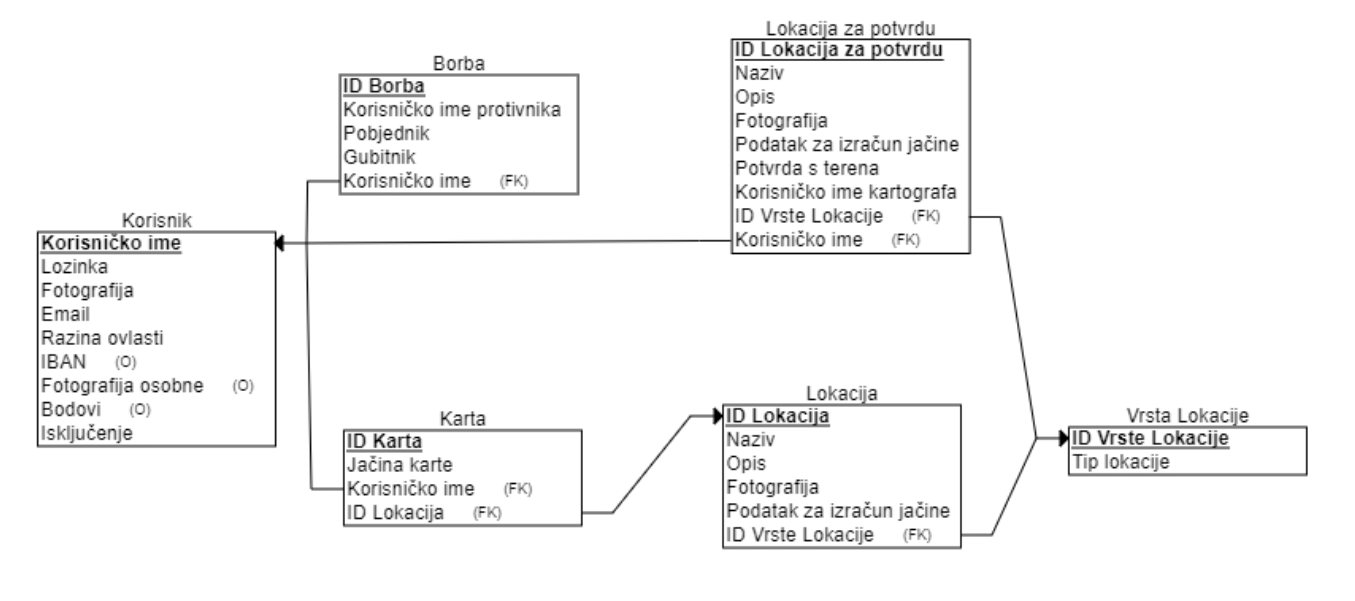
\includegraphics[width=\textwidth]{slike/Baza.PNG} %veličina slike u odnosu na originalnu datoteku i pozicija slike
					\centering
					\caption{Dijagram baze podataka}
					\label{fig:promjene}
				\end{figure}
			
			\eject
			
			
		\section{Dijagram razreda}
		
			%\textit{Potrebno je priložiti dijagram razreda s pripadajućim opisom. Zbog preglednosti je moguće dijagram razlomiti na više njih, ali moraju biti grupirani prema sličnim razinama apstrakcije i srodnim funkcionalnostima.}\\
			
			%\textbf{\textit{dio 1. revizije}}\\
			
			%\textit{Prilikom prve predaje projekta, potrebno je priložiti potpuno razrađen dijagram razreda vezan uz \textbf{generičku funkcionalnost} sustava. Ostale funkcionalnosti trebaju biti idejno razrađene u dijagramu sa sljedećim komponentama: nazivi razreda, nazivi metoda i vrste pristupa metodama (npr. javni, zaštićeni), nazivi atributa razreda, veze i odnosi između razreda.}\\

			Svaka od navedenih klasa predstavlja jednu od relacija baze podataka. Sve one nasljeđuju klasu Model. Na slici 4.4 prikazani su slojevi koji manipuliraju podacima vezanima uz korisnika - preko Controllera koji dohvaća unesene podatke preko Service klase koja ih prenosi do Repository klase koja podatke unosi u bazu i isti taj postupak obrnutim smjerom. Klase koje nasljeđuju RuntimeException koriste se kod implementacije logike upravljanja backend dijelom aplikacije te se bacaju kod raznih nedopuštenih ponašanja korisnika.
	
			 %unos slike
				\begin{figure}[H]
					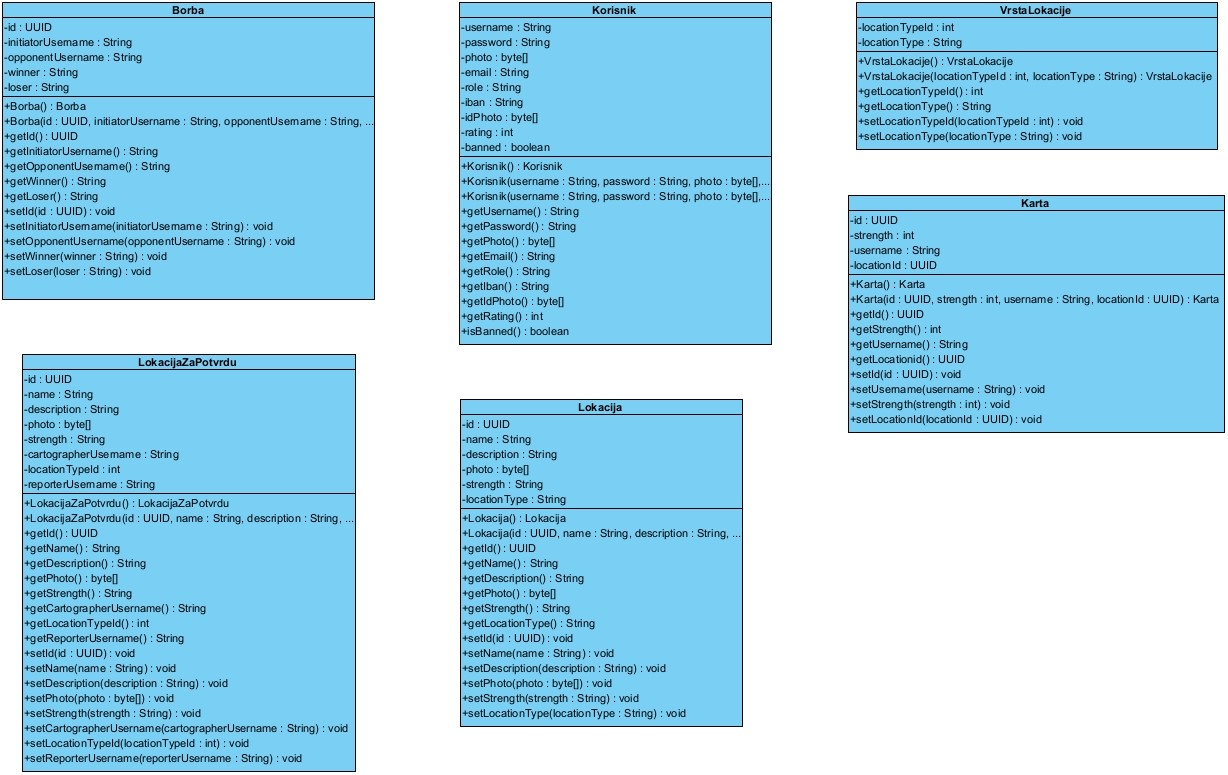
\includegraphics[width=\textwidth]{slike/model.jpg} %veličina slike u odnosu na originalnu datoteku i pozicija slike
					\centering
					\caption{Dijagram razreda - dio Model}
					\label{fig:promjene}
				\end{figure}
			\eject

			 %unos slike
				\begin{figure}[H]
					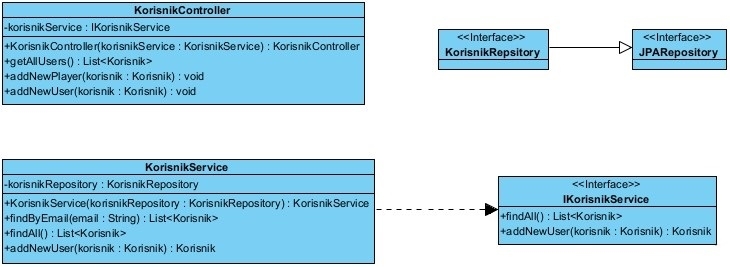
\includegraphics[width=\textwidth]{slike/service.jpg} %veličina slike u odnosu na originalnu datoteku i pozicija slike
					\centering
					\caption{Dijagram razreda - dio Service}
					\label{fig:promjene}
				\end{figure}

			 %unos slike
				\begin{figure}[H]
					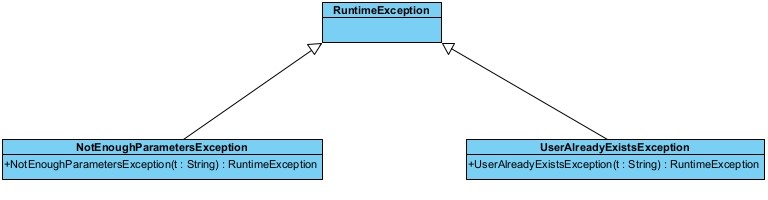
\includegraphics[width=\textwidth]{slike/exception.jpg} %veličina slike u odnosu na originalnu datoteku i pozicija slike
					\centering
					\caption{Dijagram razreda - dio Exceptions}
					\label{fig:promjene}
				\end{figure}

\iffalse
			
			\textbf{\textit{dio 2. revizije}}\\			
			
			\textit{Prilikom druge predaje projekta dijagram razreda i opisi moraju odgovarati stvarnom stanju implementacije}
			
			
			
			\eject
		
		\section{Dijagram stanja}
			
			
			\textbf{\textit{dio 2. revizije}}\\
			
			{Potrebno je priložiti dijagram stanja i opisati ga. Dovoljan je jedan dijagram stanja koji prikazuje \textbf{značajan dio funkcionalnosti} sustava. Na primjer, stanja korisničkog sučelja i tijek korištenja neke ključne funkcionalnosti jesu značajan dio sustava, a registracija i prijava nisu. }
			
			
			\eject 
		
		\section{Dijagram aktivnosti}
			
			\textbf{\textit{dio 2. revizije}}\\
			
			 \textit{Potrebno je priložiti dijagram aktivnosti s pripadajućim opisom. Dijagram aktivnosti treba prikazivati značajan dio sustava.}
			
			\eject
		\section{Dijagram komponenti}
		
			\textbf{\textit{dio 2. revizije}}\\
		
			 \textit{Potrebno je priložiti dijagram komponenti s pripadajućim opisom. Dijagram komponenti treba prikazivati strukturu cijele aplikacije.}
\fi
\iffalse
\chapter{Implementacija i korisničko sučelje}
		
		
		\section{Korištene tehnologije i alati}
		
			\textbf{\textit{dio 2. revizije}}
			
			 %\textit{Detaljno navesti sve tehnologije i alate koji su primijenjeni pri izradi dokumentacije i aplikacije. Ukratko ih opisati, te navesti njihovo značenje i mjesto primjene. Za svaki navedeni alat i tehnologiju je potrebno \textbf{navesti internet poveznicu} gdje se mogu preuzeti ili više saznati o njima}.
			
			
			\eject 
		
	
		\section{Ispitivanje programskog rješenja}
			
			\textbf{\textit{dio 2. revizije}}\\
			
			 %\textit{U ovom poglavlju je potrebno opisati provedbu ispitivanja implementiranih funkcionalnosti na razini komponenti i na razini cijelog sustava s prikazom odabranih ispitnih slučajeva. Studenti trebaju ispitati temeljnu funkcionalnost i rubne uvjete.}
	
			
			\subsection{Ispitivanje komponenti}
			%\textit{Potrebno je provesti ispitivanje jedinica (engl. unit testing) nad razredima koji implementiraju temeljne funkcionalnosti. Razraditi \textbf{minimalno 6 ispitnih slučajeva} u kojima će se ispitati redovni slučajevi, rubni uvjeti te izazivanje pogreške (engl. exception throwing). Poželjno je stvoriti i ispitni slučaj koji koristi funkcionalnosti koje nisu implementirane. Potrebno je priložiti izvorni kôd svih ispitnih slučajeva te prikaz rezultata izvođenja ispita u razvojnom okruženju (prolaz/pad ispita). }
			
			
			
			\subsection{Ispitivanje sustava}
			
			 %\textit{Potrebno je provesti i opisati ispitivanje sustava koristeći radni okvir Selenium\footnote{\url{https://www.seleniumhq.org/}}. Razraditi \textbf{minimalno 4 ispitna slučaja} u kojima će se ispitati redovni slučajevi, rubni uvjeti te poziv funkcionalnosti koja nije implementirana/izaziva pogrešku kako bi se vidjelo na koji način sustav reagira kada nešto nije u potpunosti ostvareno. Ispitni slučaj se treba sastojati od ulaza (npr. korisničko ime i lozinka), očekivanog izlaza ili rezultata, koraka ispitivanja i dobivenog izlaza ili rezultata.\\ }
			 
			\iffalse \textit{Izradu ispitnih slučajeva pomoću radnog okvira Selenium moguće je provesti pomoću jednog od sljedeća dva alata:}
			 \begin{itemize}
			 	\item \textit{dodatak za preglednik \textbf{Selenium IDE} - snimanje korisnikovih akcija radi automatskog ponavljanja ispita	}
			 	\item \textit{\textbf{Selenium WebDriver} - podrška za pisanje ispita u jezicima Java, C\#, PHP koristeći posebno programsko sučelje.}
			 \end{itemize}
		 	\textit{Detalji o korištenju alata Selenium bit će prikazani na posebnom predavanju tijekom semestra.}
			
			\eject 
            \fi
		
		
		\section{Dijagram razmještaja}
			
			\textbf{\textit{dio 2. revizije}}
			
			% \textit{Potrebno je umetnuti \textbf{specifikacijski} dijagram razmještaja i opisati ga. Moguće je umjesto specifikacijskog dijagrama razmještaja umetnuti dijagram razmještaja instanci, pod uvjetom da taj dijagram bolje opisuje neki važniji dio sustava.}
			
			\eject 
		
		\section{Upute za puštanje u pogon}
		
			\textbf{\textit{dio 2. revizije}}\\
		
			% \textit{U ovom poglavlju potrebno je dati upute za puštanje u pogon (engl. deployment) ostvarene aplikacije. Na primjer, za web aplikacije, opisati postupak kojim se od izvornog kôda dolazi do potpuno postavljene baze podataka i poslužitelja koji odgovara na upite korisnika. Za mobilnu aplikaciju, postupak kojim se aplikacija izgradi, te postavi na neku od trgovina. Za stolnu (engl. desktop) aplikaciju, postupak kojim se aplikacija instalira na računalo. Ukoliko mobilne i stolne aplikacije komuniciraju s poslužiteljem i/ili bazom podataka, opisati i postupak njihovog postavljanja. Pri izradi uputa preporučuje se \textbf{naglasiti korake instalacije uporabom natuknica} te koristiti što je više moguće \textbf{slike ekrana} (engl. screenshots) kako bi upute bile jasne i jednostavne za slijediti.}
			
			
			% \textit{Dovršenu aplikaciju potrebno je pokrenuti na javno dostupnom poslužitelju. Studentima se preporuča korištenje neke od sljedećih besplatnih usluga: \href{https://aws.amazon.com/}{Amazon AWS}, \href{https://azure.microsoft.com/en-us/}{Microsoft Azure} ili \href{https://www.heroku.com/}{Heroku}. Mobilne aplikacije trebaju biti objavljene na F-Droid, Google Play ili Amazon App trgovini.}
			
			
			\eject
\fi
%\chapter{Zaključak i budući rad}
		
		%\textbf{\textit{dio 2. revizije}}\\
		
		 %\textit{U ovom poglavlju potrebno je napisati osvrt na vrijeme izrade projektnog zadatka, koji su tehnički izazovi prepoznati, jesu li riješeni ili kako bi mogli biti riješeni, koja su znanja stečena pri izradi projekta, koja bi znanja bila posebno potrebna za brže i kvalitetnije ostvarenje projekta i koje bi bile perspektive za nastavak rada u projektnoj grupi.}
		
		% \textit{Potrebno je točno popisati funkcionalnosti koje nisu implementirane u ostvarenoj aplikaciji.}
		
		%\eject 
\chapter*{Popis literature}
		\addcontentsline{toc}{chapter}{Popis literature}
	 	
 		%\textbf{\textit{Kontinuirano osvježavanje}}
	
		%\textit{Popisati sve reference i literaturu koja je pomogla pri ostvarivanju projekta.}
		
		
		\begin{enumerate}
			
			
			\item  Programsko inženjerstvo, FER ZEMRIS, \url{http://www.fer.hr/predmet/proinz}
			
			\item  I. Sommerville, "Software engineering", 8th ed, Addison Wesley, 2007.
			
			\item  T.C.Lethbridge, R.Langaniere, "Object-Oriented Software Engineering", 2nd ed. McGraw-Hill, 2005.
			
			\item  I. Marsic, Software engineering book``, Department of Electrical and Computer Engineering, Rutgers University, \url{http://www.ece.rutgers.edu/~marsic/books/SE}
			
			\item  The Unified Modeling Language, \url{https://www.uml-diagrams.org/}
			
			\item  Astah Community, \url{http://astah.net/editions/uml-new}
		\end{enumerate}
		
		 


\begingroup
\renewcommand*\listfigurename{Indeks slika i dijagrama}
%\renewcommand*\listtablename{Indeks tablica}
%\let\clearpage\relax
\listoffigures
%\vspace{10mm}
%\listoftables
\endgroup
\addcontentsline{toc}{chapter}{Indeks slika i dijagrama}



\eject 

\chapter*{Dodatak: Prikaz aktivnosti grupe}
		\addcontentsline{toc}{chapter}{Dodatak: Prikaz aktivnosti grupe}
		
		\section*{Dnevnik sastajanja}
		
		%\textbf{\textit{Kontinuirano osvježavanje}}\\
		
		 %\textit{U ovom dijelu potrebno je redovito osvježavati dnevnik sastajanja prema predlošku.}
		
		\begin{packed_enum}
			\item  sastanak
			\item[] \begin{packed_item}
				\item Datum: 20.listopada 2022.
				\item Prisustvovali: L.Arambašić, M.Arambašić, M.Kopačević, R.Kunštek, D.Smolić-Ročak
				\item Teme sastanka:
				\begin{packed_item}
					\item  odabir tehnologija
					\item  generalna rasprava o zadatku s asistentom
				\end{packed_item}
			\end{packed_item}
			
			\item  sastanak
			\item[] \begin{packed_item}
				\item Datum: 1.studenoga 2022.
				\item Prisustvovali: L.Arambašić, M.Arambašić, M.Krapanić, R.Kunštek, D.Smolić-Ročak
				\item Teme sastanka:
				\begin{packed_item}
					\item  razmatranje poglavlja dokumentacije
					\item  razmatranje potrebnih UC dijagrama
				\end{packed_item}
			\end{packed_item}
		
			\item  sastanak
			\item[] \begin{packed_item}
				\item Datum: 6.studenoga 2022.
				\item Prisustvovali: L.Arambašić, M.Arambašić, M.Krapanić, M.Kopačević, R.Kunštek, D.Smolić-Ročak
				\item Teme sastanka:
				\begin{packed_item}
					\item  revizija UC dijagrama
					\item  rasprava implementacije borbe
				\end{packed_item}
			\end{packed_item}
		
			\item  sastanak
			\item[] \begin{packed_item}
				\item Datum: 10.studenoga 2022.
				\item Prisustvovali: L.Arambašić, M.Kopačević, R.Kunštek
				\item Teme sastanka:
				\begin{packed_item}
					\item  rasprava oko detalja dokumentacije i funkcionalnosti v1 s asistentom i demonstratorom
				\end{packed_item}
			\end{packed_item}
		
			\item  sastanak
			\item[] \begin{packed_item}
				\item Datum: 16.studenoga 2022.
				\item Prisustvovali: L.Arambašić, M.Arambašić, M.Krapanić, M.Kopačević, R.Kunštek, D.Smolić-Ročak
				\item Teme sastanka:
				\begin{packed_item}
					\item  revizija dokumentacije v1 
					\item  revizija generalne funkcionalnosti programa
				\end{packed_item}
			\end{packed_item}
			
			%
			
		\end{packed_enum}
		
		\eject
		\section*{Tablica aktivnosti}
		
			\textbf{\textit{Kontinuirano osvježavanje}}\\
			
			 %\textit{Napomena: Doprinose u aktivnostima treba navesti u satima po članovima grupe po aktivnosti.}

			\begin{longtblr}[
					label=none,
				]{
					vlines,hlines,
					width = \textwidth,
					colspec={X[7, l]X[1, c]X[1, c]X[1, c]X[1, c]X[1, c]X[1, c]X[1, c]}, 
					vline{1} = {1}{text=\clap{}},
					hline{1} = {1}{text=\clap{}},
					rowhead = 1,
				} 
				\SetCell[c=1]{r}{} & \SetCell[c=1]{r}{\rotatebox{90}{\textbf{Robert Kunštek}}} & \SetCell[c=1]{r}{\rotatebox{90}{\textbf{Luka Arambašić }}} & \SetCell[c=1]{r}{\rotatebox{90}{\textbf{Marela Arambašić }}} & \SetCell[c=1]{r}{\rotatebox{90}{\textbf{Mateo Kopačević }}} &	\SetCell[c=1]{r}{\rotatebox{90}{\textbf{Marin Krapanić }}} & 	\SetCell[c=1]{r}{\rotatebox{90}{\textbf{Damjan Smolić-Ročak }}} \\  
				Upravljanje projektom 		&  &  &  &  &  &  & \\ 
				Opis projektnog zadatka 	&  &  &  &  &  &  & \\ 
				
				Funkcionalni zahtjevi       &  &  &  &  &  &  &  \\ 
				Opis pojedinih obrazaca 	&  &  &  &  &  &  &  \\ 
				Dijagram obrazaca 			&  &  &  &  &  &  &  \\ 
				Sekvencijski dijagrami 		&  &  &  &  &  &  &  \\ 
				Opis ostalih zahtjeva 		&  &  &  &  &  &  &  \\ 

				Arhitektura i dizajn sustava	 &  &  &  &  &  &  &  \\ 
				Baza podataka				&  &  &  &  &  &  &   \\ 
				Dijagram razreda 			&  &  &  &  &  &  &   \\ 
				Dijagram stanja				&  &  &  &  &  &  &  \\ 
				Dijagram aktivnosti 		&  &  &  &  &  &  &  \\ 
				Dijagram komponenti			&  &  &  &  &  &  &  \\ 
				Korištene tehnologije i alati 		&  &  &  &  &  &  &  \\ 
				Ispitivanje programskog rješenja 	&  &  &  &  &  &  &  \\ 
				Dijagram razmještaja			&  &  &  &  &  &  &  \\ 
				Upute za puštanje u pogon 		&  &  &  &  &  &  &  \\  
				Dnevnik sastajanja 			&  &  &  &  &  &  &  \\ 
				Zaključak i budući rad 		&  &  &  &  &  &  &  \\  
				Popis literature 			&  &  &  &  &  &  &  \\  
				&  &  &  &  &  &  &  \\ \hline 
				\textit{Dodatne stavke kako ste podijelili izradu aplikacije} 			&  &  &  &  &  &  &  \\ 
				\textit{npr. izrada početne stranice} 				&  &  &  &  &  &  &  \\  
				\textit{izrada baze podataka} 		 			&  &  &  &  &  &  & \\  
				\textit{spajanje s bazom podataka} 							&  &  &  &  &  &  &  \\ 
				\textit{back end} 							&  &  &  &  &  &  &  \\  
				 							&  &  &  &  &  &  &\\ 
			\end{longtblr}
					
					
		\eject
		%\section*{Dijagrami pregleda promjena}
		
		%\textbf{\textit{dio 2. revizije}}\\
		
		%\textit{Prenijeti dijagram pregleda promjena nad datotekama projekta. Potrebno je na kraju projekta generirane grafove s gitlaba prenijeti u ovo poglavlje dokumentacije. Dijagrami za vlastiti projekt se mogu preuzeti s gitlab.com stranice, u izborniku Repository, pritiskom na stavku Contributors.}
		
	


\end{document} %naredbe i tekst nakon ove naredbe ne ulaze u izgrađen dokument 